\documentclass[14pt]{book}

\usepackage{fancyhdr}
\usepackage{graphicx}
\usepackage[margin=2.5cm]{geometry}
\usepackage{graphicx}
\usepackage{anysize}
\usepackage{xcolor}
\usepackage{caption}
\usepackage{subcaption}

\marginsize{2cm}{2cm}{2cm}{2cm} % Izquierda, derecha, arriba, abajo
\setlength{\parindent}{0cm}
\pagestyle{fancy}
\fancyhf{}
\fancyhead[L]{\footnotesize Redes de computadoras} %encabezado izquierda
\fancyhead[R]{\footnotesize David Pérez Jacome}   % derecha
\fancyfoot[L]{\footnotesize}  %izquierda
\fancyfoot[C]{Página \thepage}
\renewcommand{\footrulewidth}{0.4pt}

\begin{document}
\begin{center}
  \newcommand{\HRule}{\rule{\linewidth}{0.5mm}}
  \begin{minipage}{0.48\textwidth}
    \begin{flushleft}
      
\includegraphics[scale = 0.08]{images/logo_unam.png}
    \end{flushleft}
  \end{minipage}
  \begin{minipage}{0.48\textwidth}
    \begin{flushright}
      
\includegraphics[scale =0.22]{images/logo_ciencias.png}
    \end{flushright}
  \end{minipage}
  \vspace*{-1.5cm}
  \textsc{\huge Nacional Autónoma de México \\ \vspace{-4px} Universidad }\\[2cm]
  \textsc{\LARGE Facultad de Ciencias}\\[1.5cm]
  \begin{minipage}{0.9\textwidth}
    \begin{center}
      \textsc{\LARGE Redes de computadoras}
    \end{center}
  \end{minipage}\\[0.5cm]
  \vspace*{1cm}
  \HRule \\[0.4cm]
  { \huge \bfseries Practica 06}\\[0.4cm]
  \HRule \\[1.5cm]
  \begin{minipage}{0.52\textwidth}
    \begin{flushleft} \large \small \vspace{-0.6cm} \vspace{-0.6cm}
      Alumno David Pérez Jacome \\
    \end{flushleft}
  \end{minipage}
  \begin{minipage}{0.46\textwidth}
    \vspace{-0.6cm}
    \begin{flushright} \large \small \emph{Profesor:}
      Paulo Santiago de Jesús Contreras Flores \\
    \end{flushright}
  \end{minipage}
  \vspace*{1cm}
  \vspace{2cm}
  \begin{center}
    {\large 2023}
  \end{center}
\end{center}
\newpage

{\color{blue} \section*{\textbf{Practica 06}}}
\vspace{1em}

{\color{red} \subsection*{\textbf{Ruteo dinámico con RIPv2}}}
\vspace{1em}

{\color{red} \subsection*{\textbf{Objetivo}}}
\vspace{1em}

\begin{enumerate}
  \item El alumno aprenderá el uso del software de simulación de redes Packet Tracer.
  \item Configurará rutas dinámicas usando el protocolo RIP, en los router de diferentes redes.
  \item Configurará servidores DNS de diferentes dominios para que se comuniquen entre ellos.
\end{enumerate}

{\color{red} \subsection*{\textbf{Introducción}}}
\vspace{1em}

El Routing Information Protocol \textbf{(RIP)} es un protocolo de enrutamiento dinámico que utiliza el
recuento de saltos como métrica de enrutamiento para encontrar la mejor ruta entre la red de
origen y la de destino. Funciona en la capa de aplicación del modelo OSI y utiliza el puerto 520.
Es uno de los protocolos de enrutamiento más viejos, lo que conlleva a que se utilice en redes que
se conforman por dispositivos antiguos.\\

El recuento de saltos equivale al número de routers por los que tenga que pasar la información
entre la red de origen y la de destino. De esto se concluye que la ruta con el menor número de saltos
es la mejor ruta para llegar a una red, por lo que se coloca en la tabla de enrutamiento. Pero como
todo protocolo tiene un limite en la cantidad de saltos que pueden existir para alcanzar una red,
el recuento de saltos máximo permitido es 15; si en una ruta hubiera un recuento de 16 saltos (o
más) se considerará que al red es inalcanzable. Gracias a esto RIP evita los bucles de enrutamiento
en la ruta.\\

RIP envia las actualizaciones de la red cada 30 segundos. Lo importante aqui es que estas
actualizaciones se envian a todos los componentes de la red en la que se ha configurado el protocolo;
es decir, se realiza por medio de un broadcast.\\

Finalmente, recapitulemos cuales son las principales caracteristicas de este protocolo:\\

\begin{enumerate}
  \item Las actualizaciones (información de enrutamiento) de la red se intercambian periódicamente.
  \item Las actualizaciones siempre se transmiten por medio de un broadcast.
  \item Siempre se envian las tablas de enrutamiento completas en las actualizaciones.
  \item Los routers siempre confían en la información de enrutamiento recibida de sus routers vecinos.
\end{enumerate}

\vspace{2em}

{\color{red} \subsection*{\textbf{Desarrollo}}}
\vspace{1em}

Para comenzar esta practica vamos a configurar nuevas infraestructuras, una para la red de Google:\\

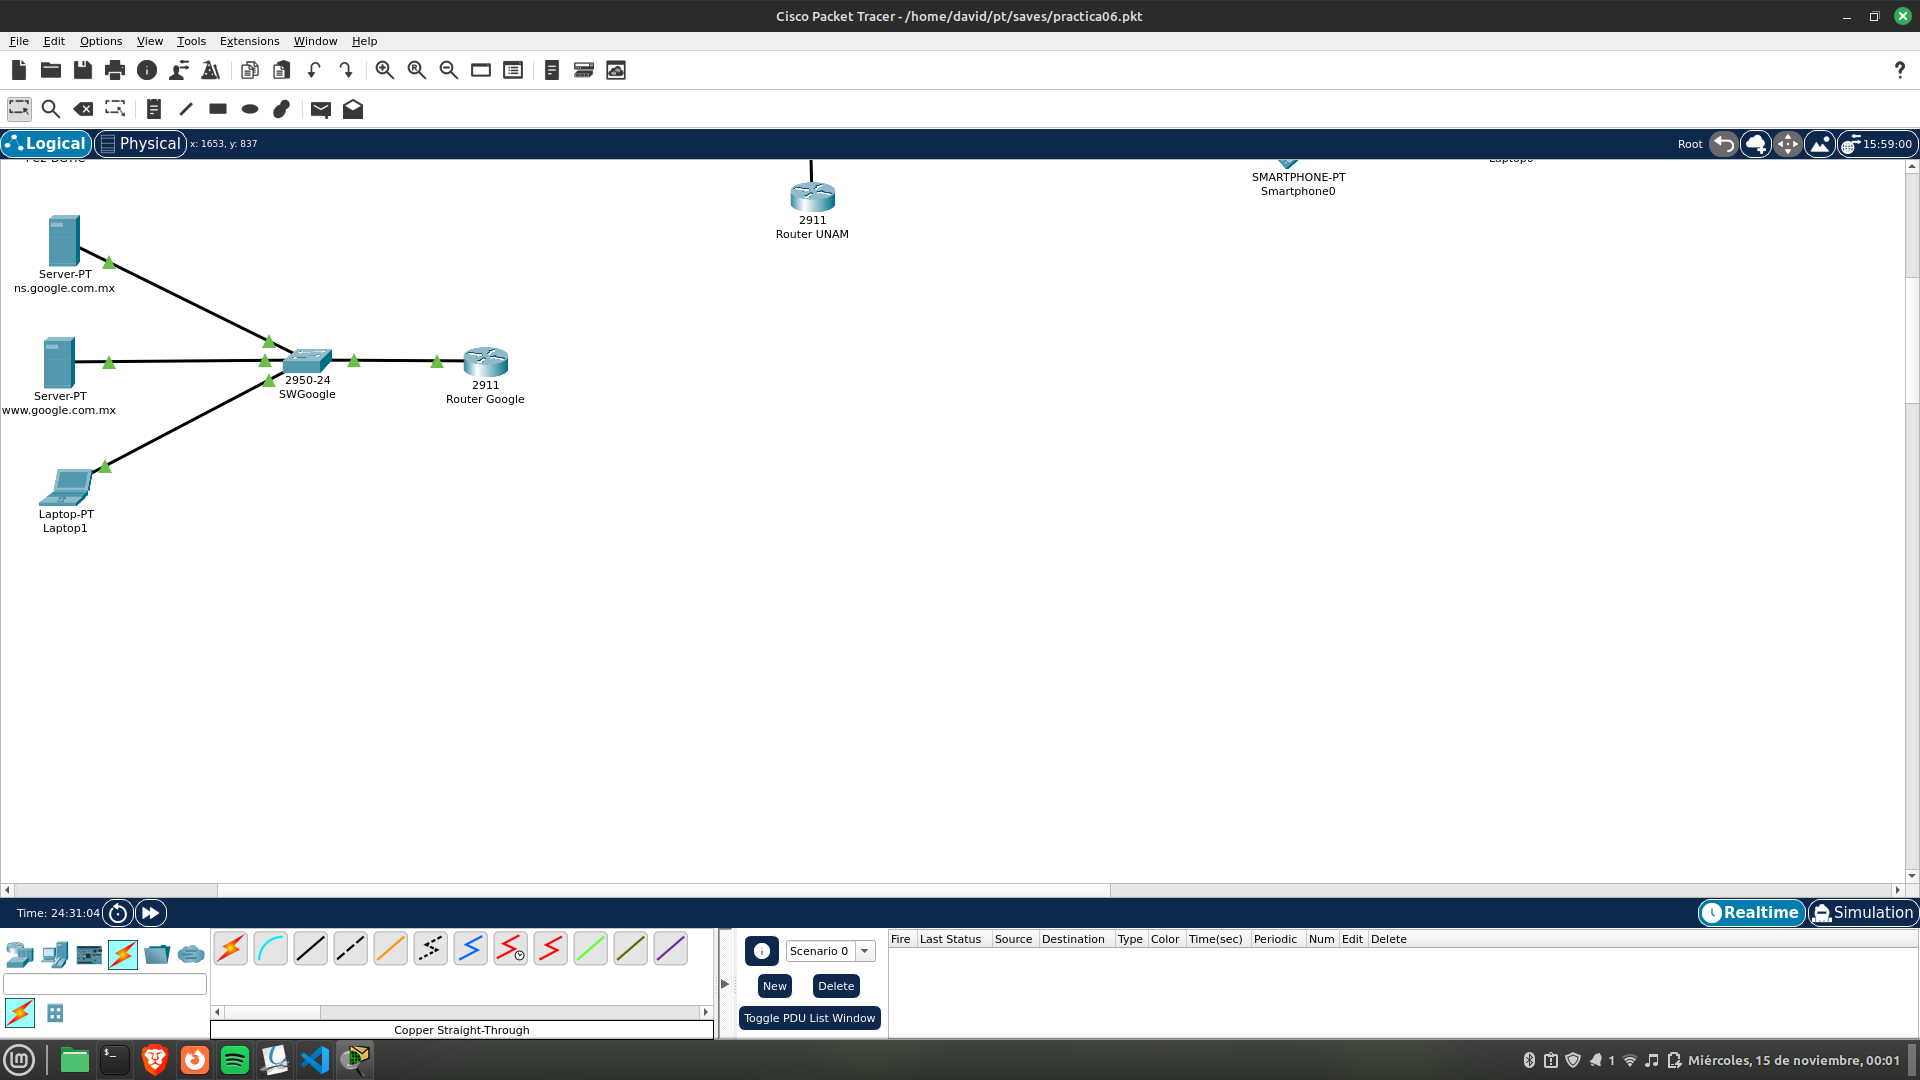
\includegraphics[width=12cm, height=8cm]{images/redgoogle.png}\\

Otra para la red de Telmex-Infinitum:\\

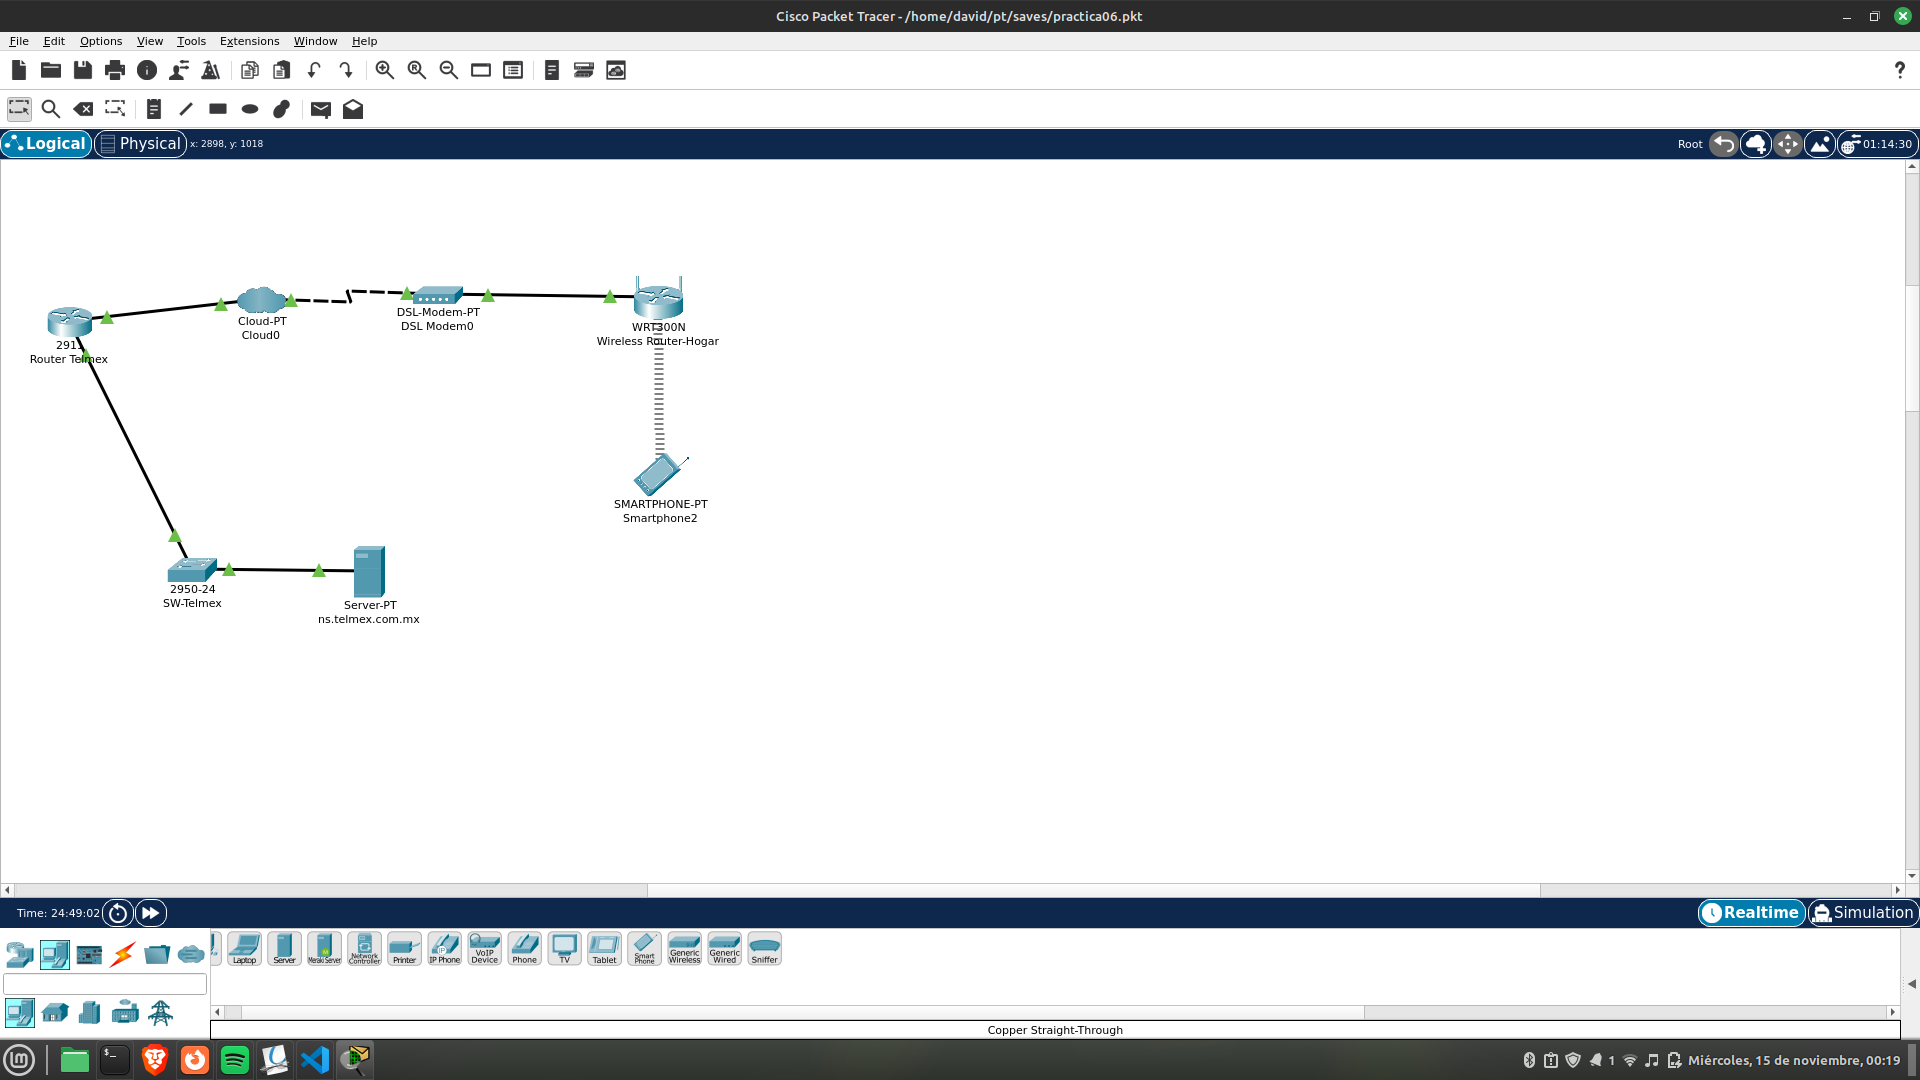
\includegraphics[width=12cm, height=8cm]{images/telmexred.png}\\

Por ahora solamente me guie de las capturas iniciales del pdf para mostrar las capturas anteriores, ahora vamos a configurar los respectivos dispositivos, iniciando con la red de Google MX.\\

Para iniciar vamos a configurar \textbf{ns.google.com.mx}, que es un servidor DNS asi que usamos las configuraciones correspondientes como activar el apartado de DNS, y desactivar HTTP, HTTPS. ademas de que como antes mencione ya habia agregado la IP y habia hecho las conexiones,
solamente tuve que configurar en los 3 dispositivos, el Gateway y DNS-Server como se muestra a continuación:\\

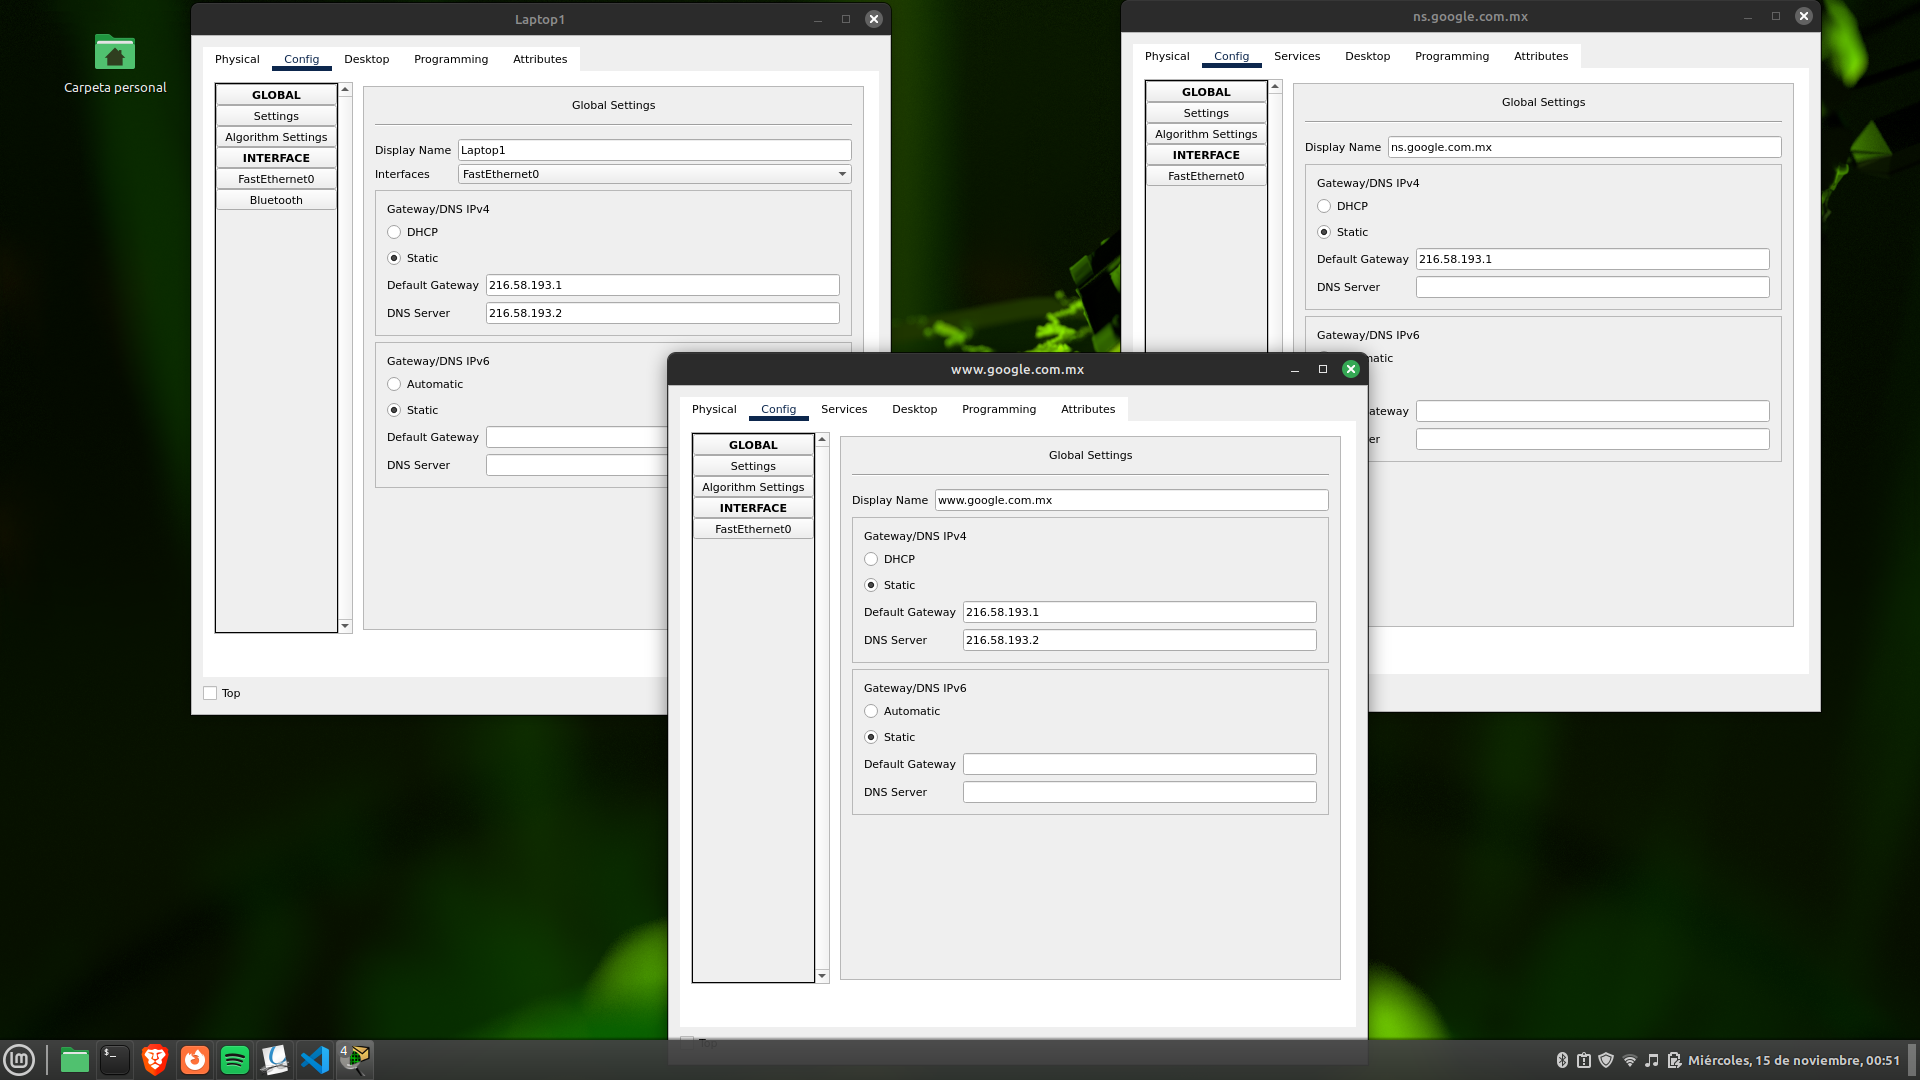
\includegraphics[width=12cm, height=8cm]{images/dnsconfiguaracion.png}\\

De igual manera configuramos el \textbf{ns.telmex.com.mx}:\\

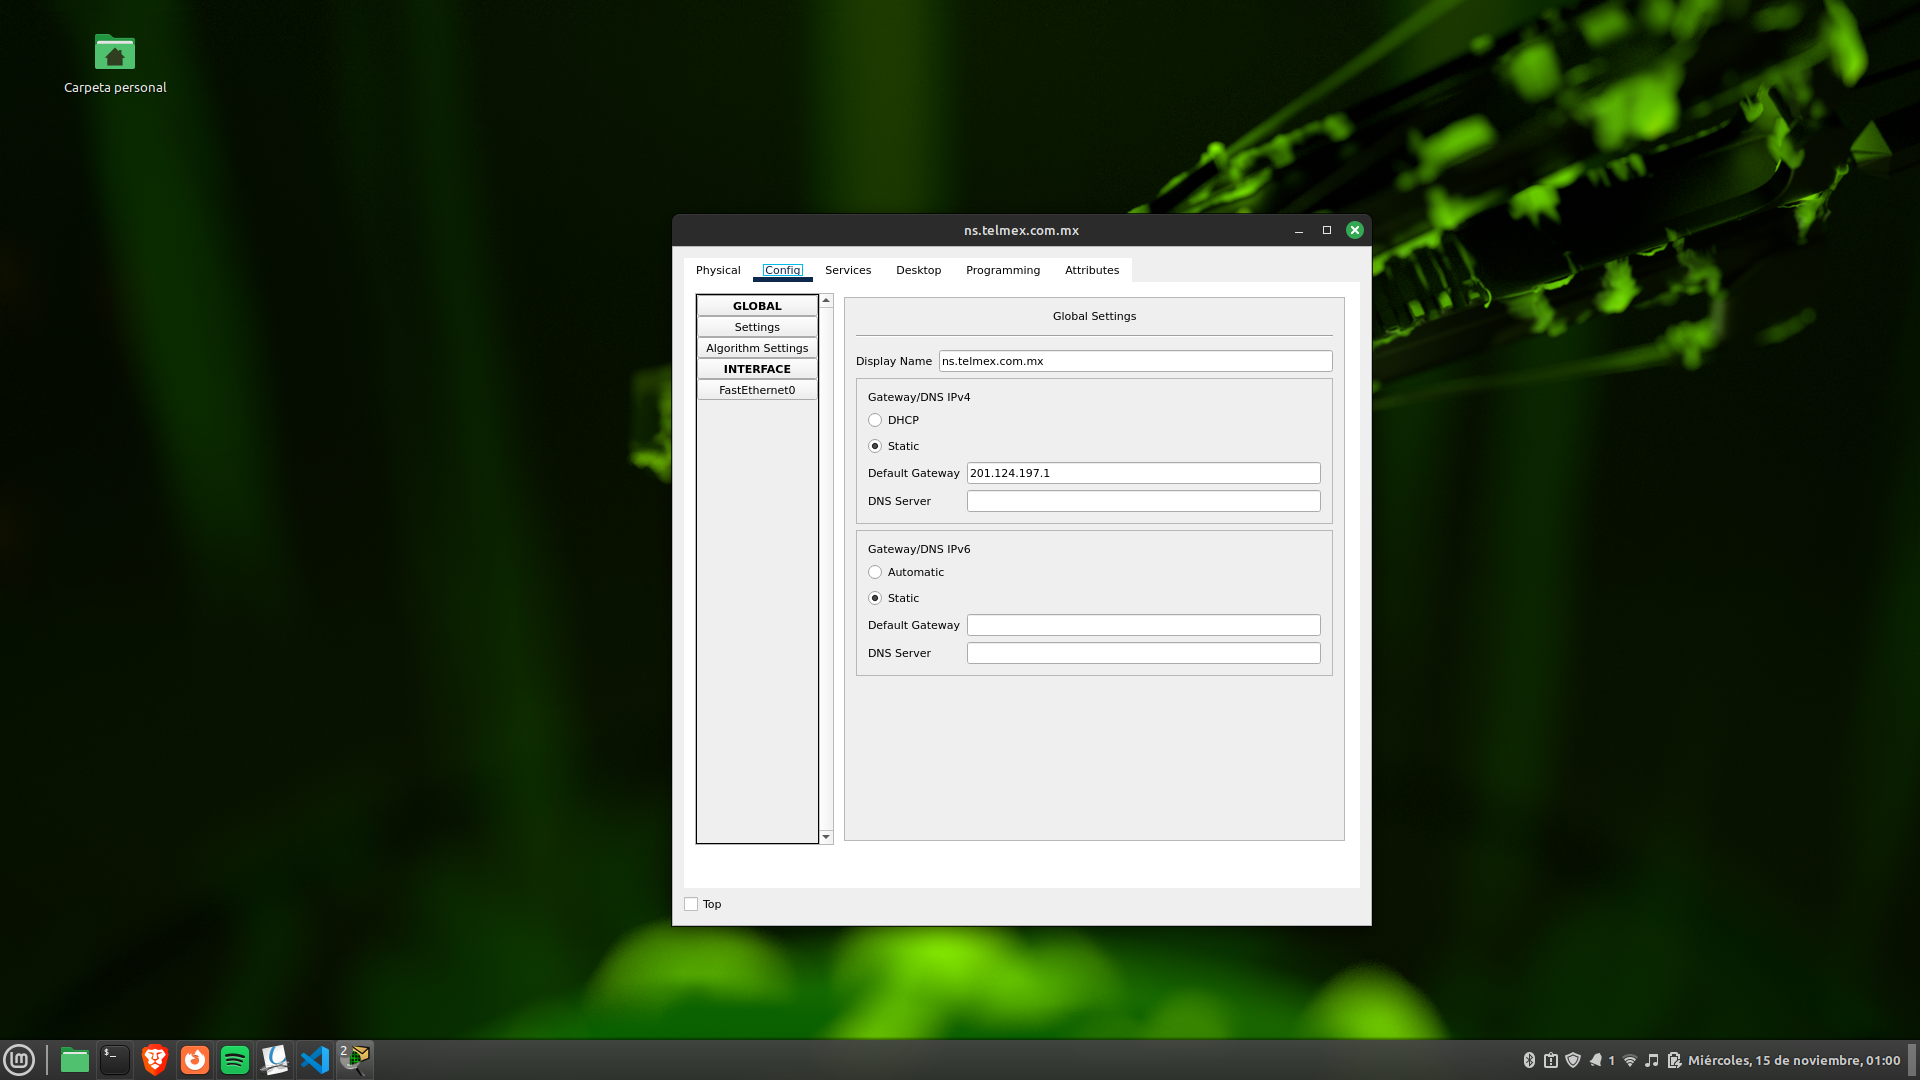
\includegraphics[width=12cm, height=8cm]{images/dnstelmex.png}\\

Ahora vamos a configurar el \textbf{Wireless Router-Hogar} similar a como lo configuramos el \textbf{RIU} más lo que nos especifica la tabla de las intrucciones del pdf.\\

Iniciamos con el \textbf{Internet Setup y Network Setup}:\\

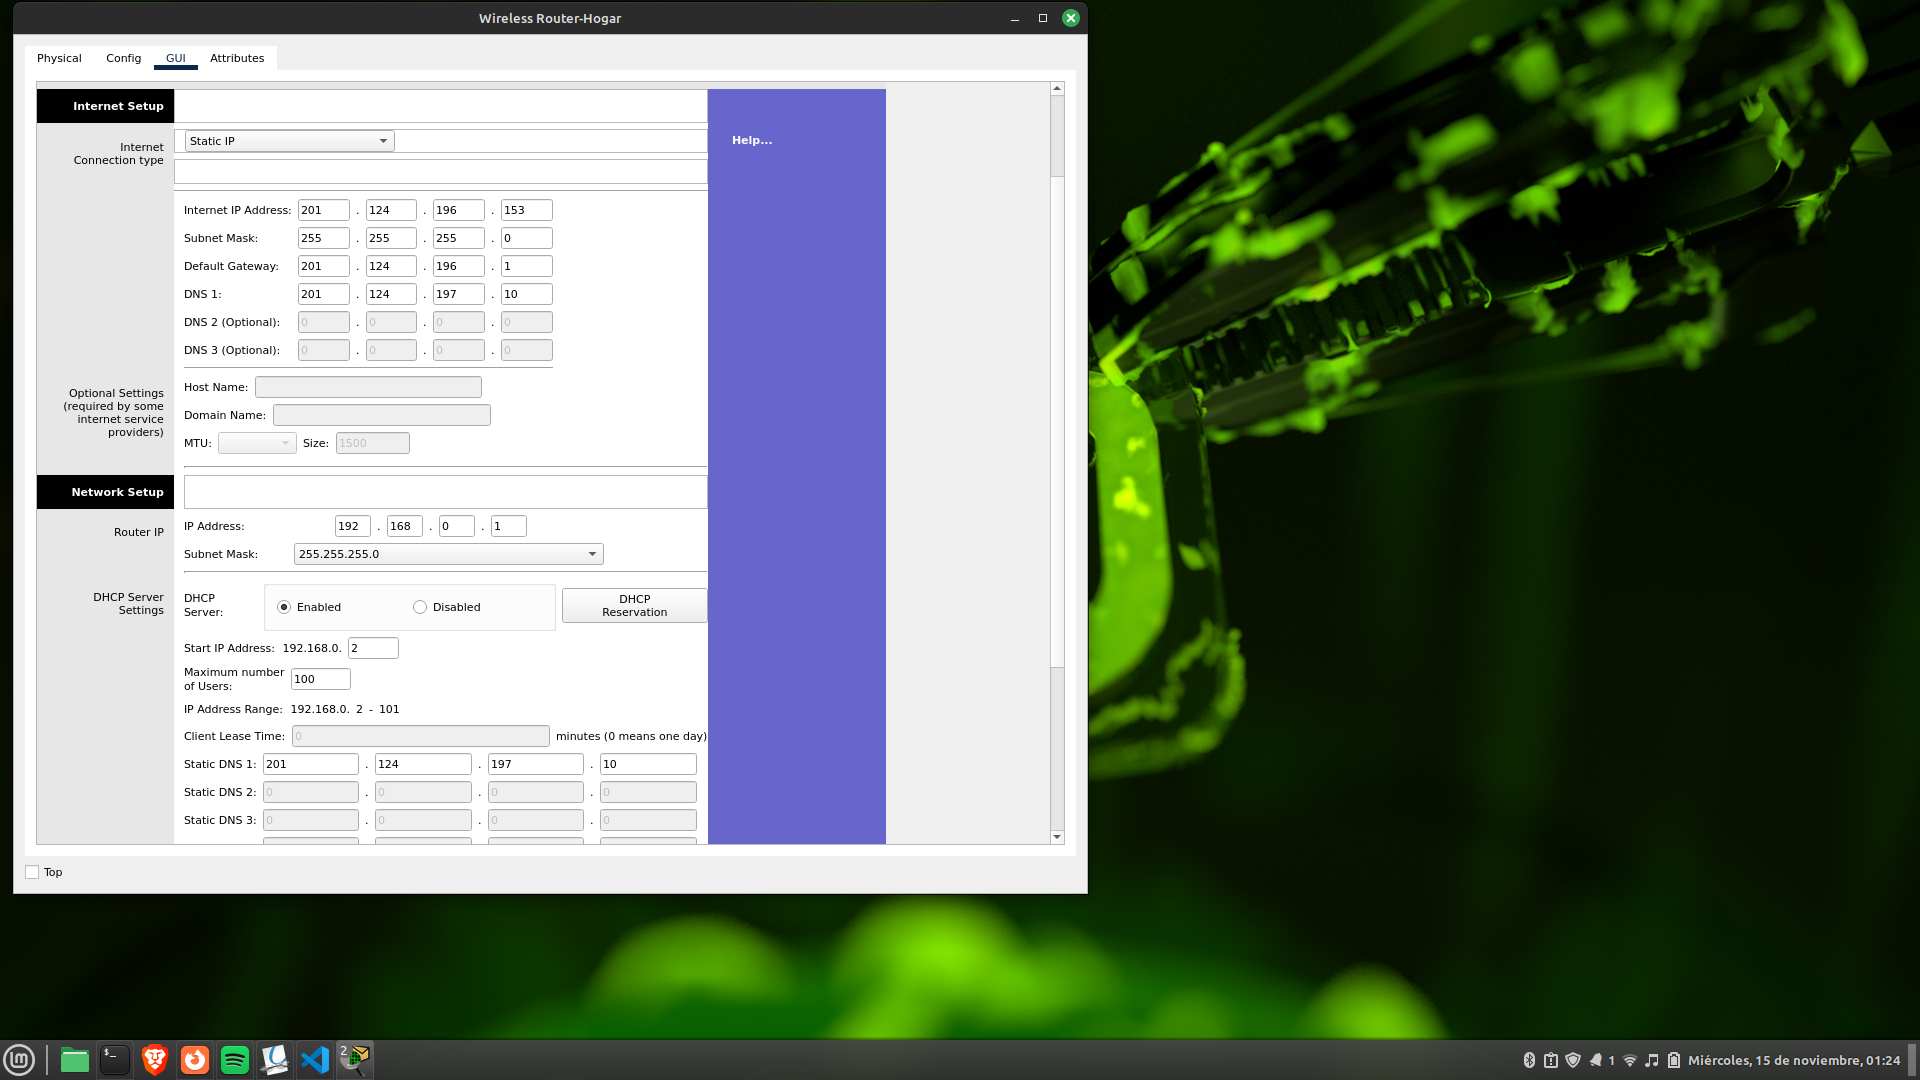
\includegraphics[width=12cm, height=8cm]{images/confiwireles.png}\\

Ahora \textbf{Basic Wireless Settings} simplemente menciono que le cambiamos el nombre a \textsf{Infinitum5678}.\\

Ahora vamos a conectar el \textbf{ Smartphone2} a esta red mencionada:\\

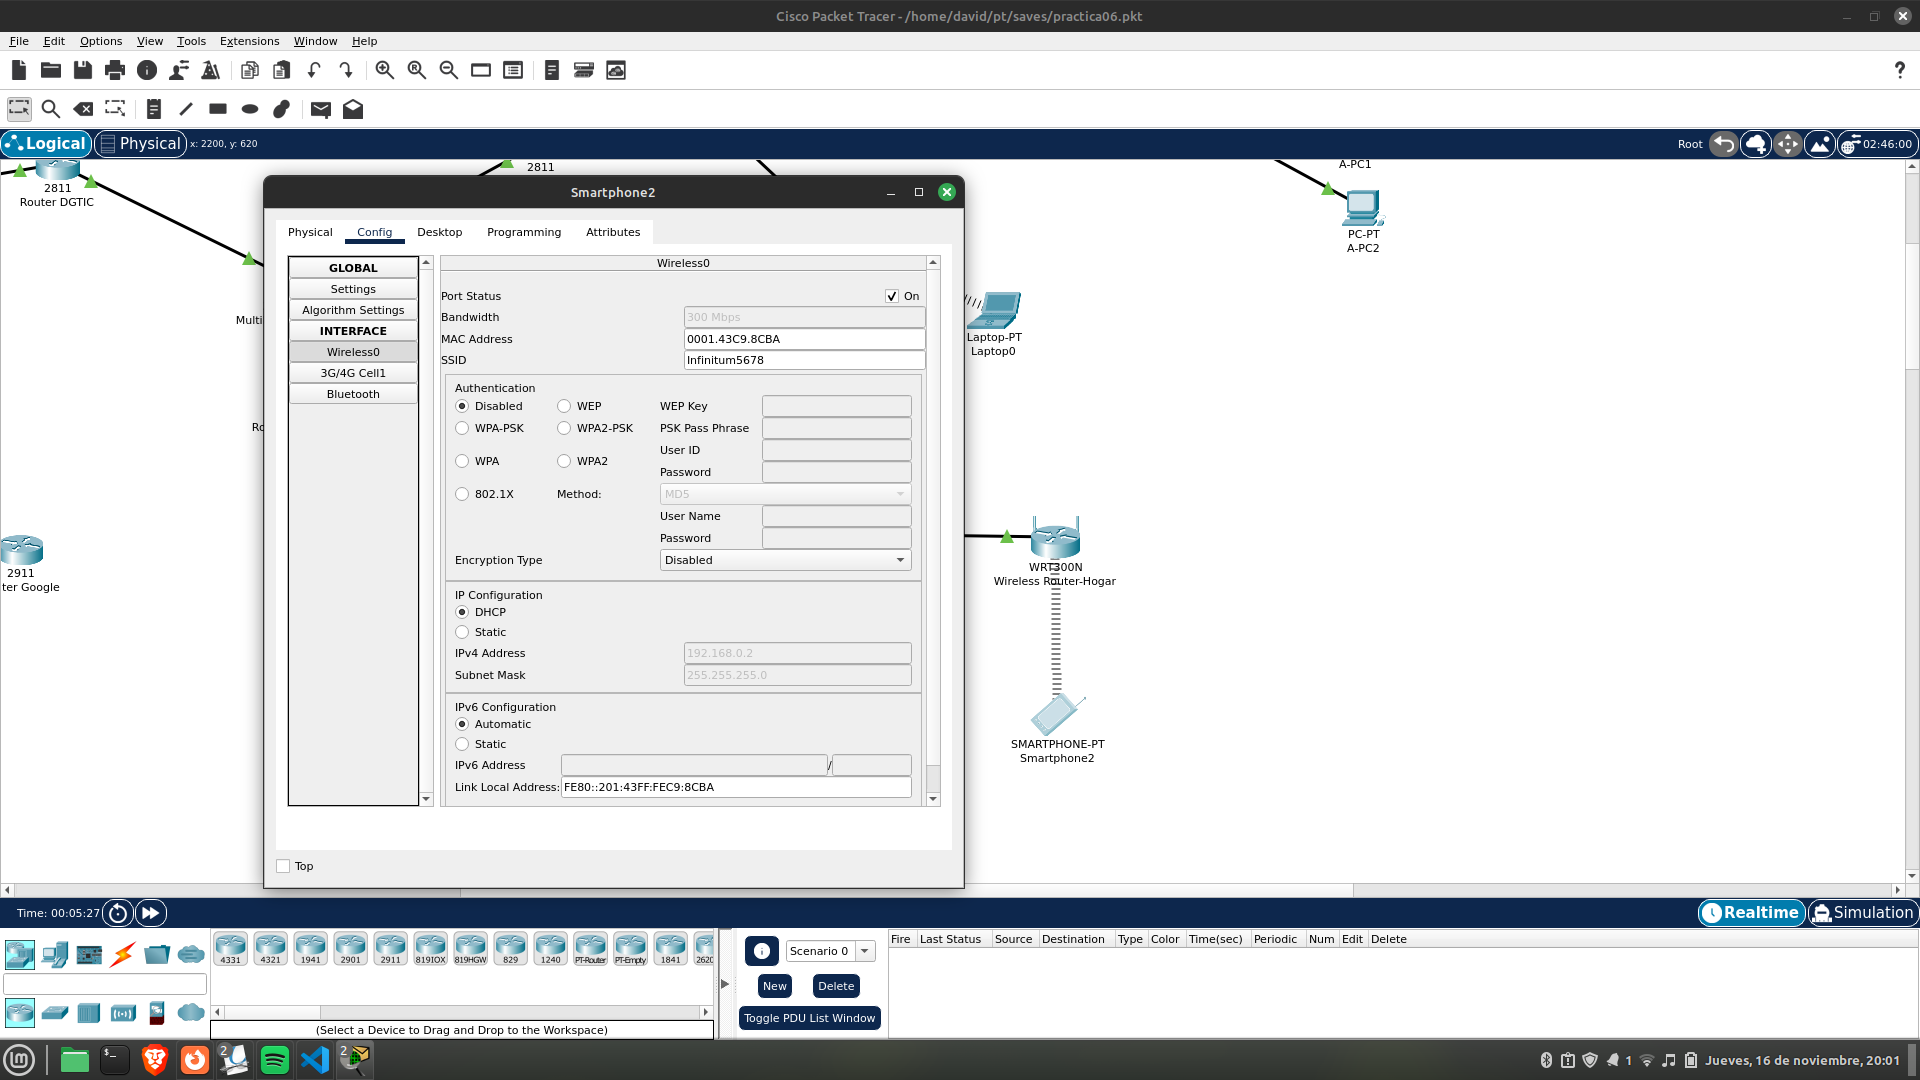
\includegraphics[width=12cm, height=8cm]{images/cel a red.png}\\

Configuaramos la nube de la siguiente manera:\\

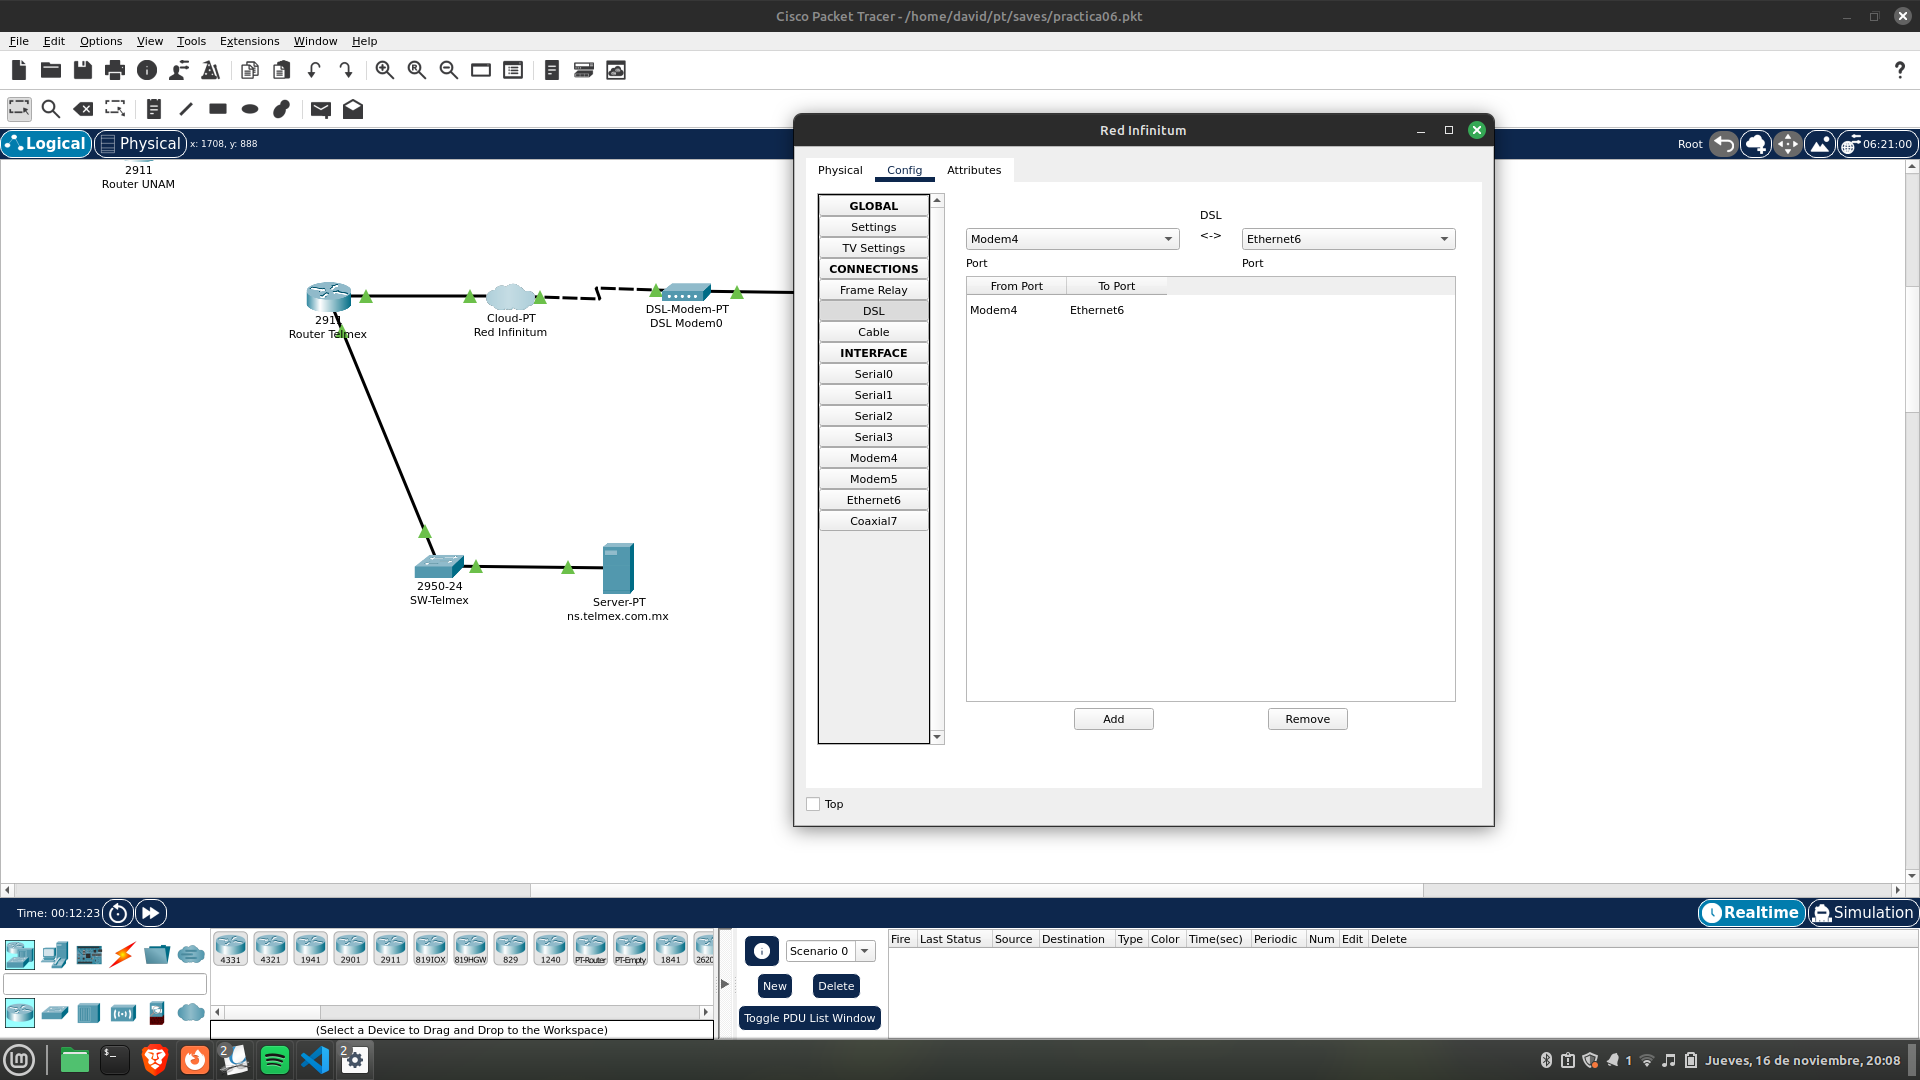
\includegraphics[width=12cm, height=8cm]{images/conf de cloud.png}\\

Seguimos con la \textbf{Configuración del sitio web de Google}:\\

El cual vamos a configurar de la misma manera que lo hicimos para el servidor de la red de la UNAM, con la diferencia que aparecerá en el index la etiqueda de "Google".\\

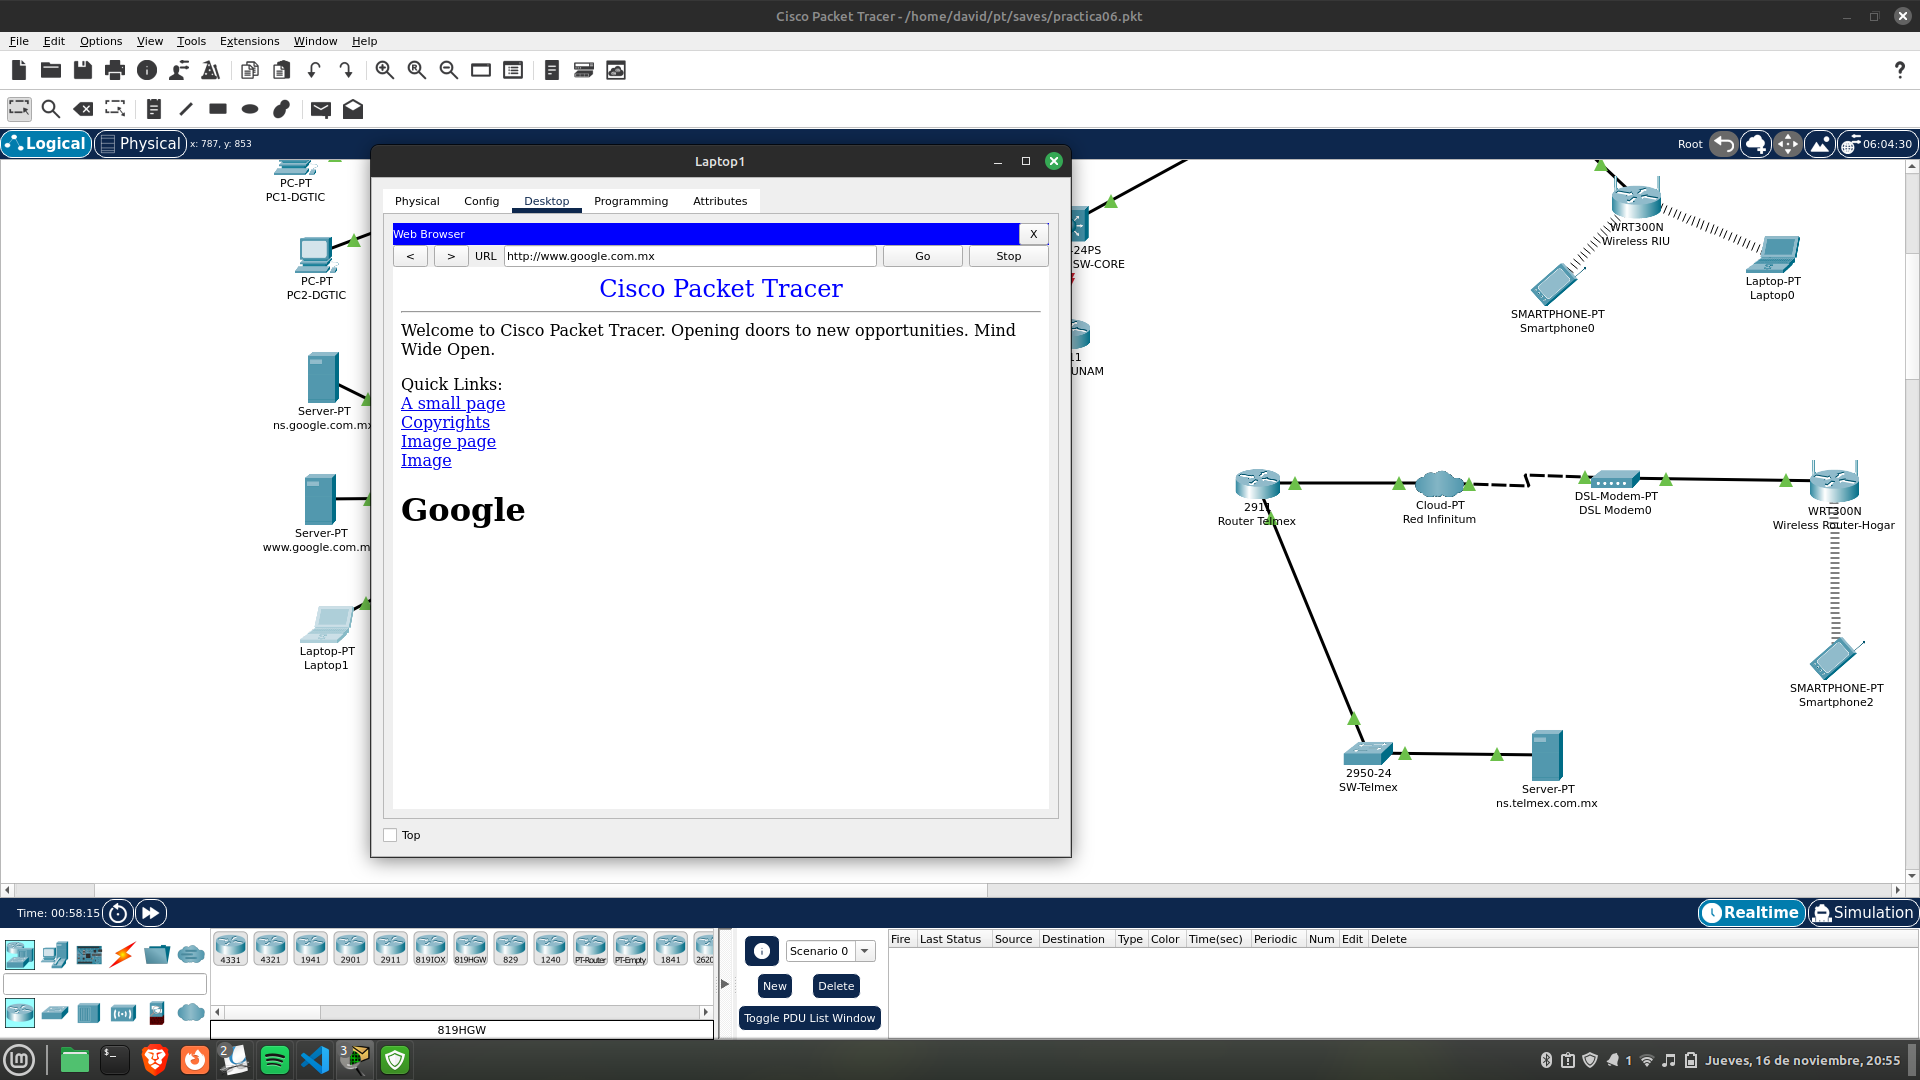
\includegraphics[width=12cm, height=8cm]{images/buscador de lab.png}\\

Ahora empezamos configurando los servidores DNS, siguiendo los pasos de la practica anterior, para el DNS de google nos queda de la siguiente manera:\\

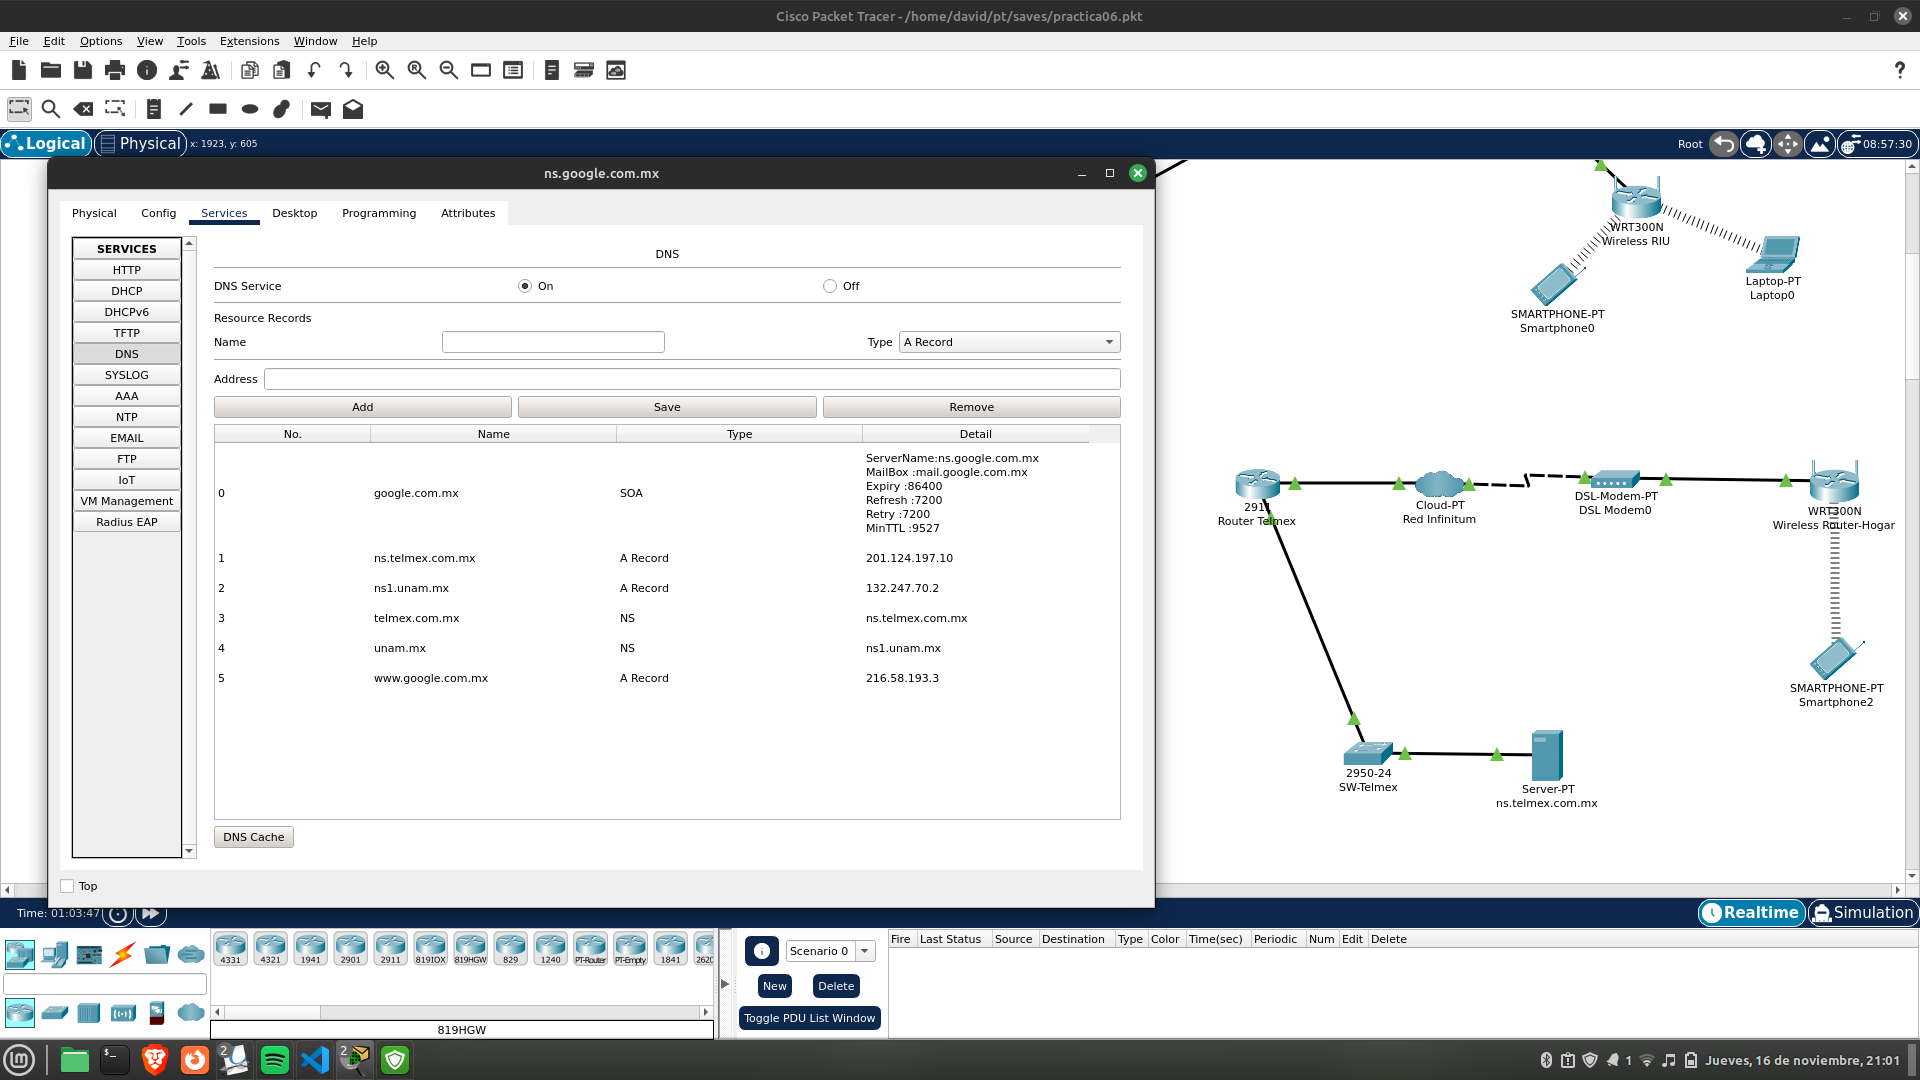
\includegraphics[width=12cm, height=8cm]{images/dns_google.png}\\

Seguimos con la configuración de \textbf{DNS Telmex-Infinitum}:\\

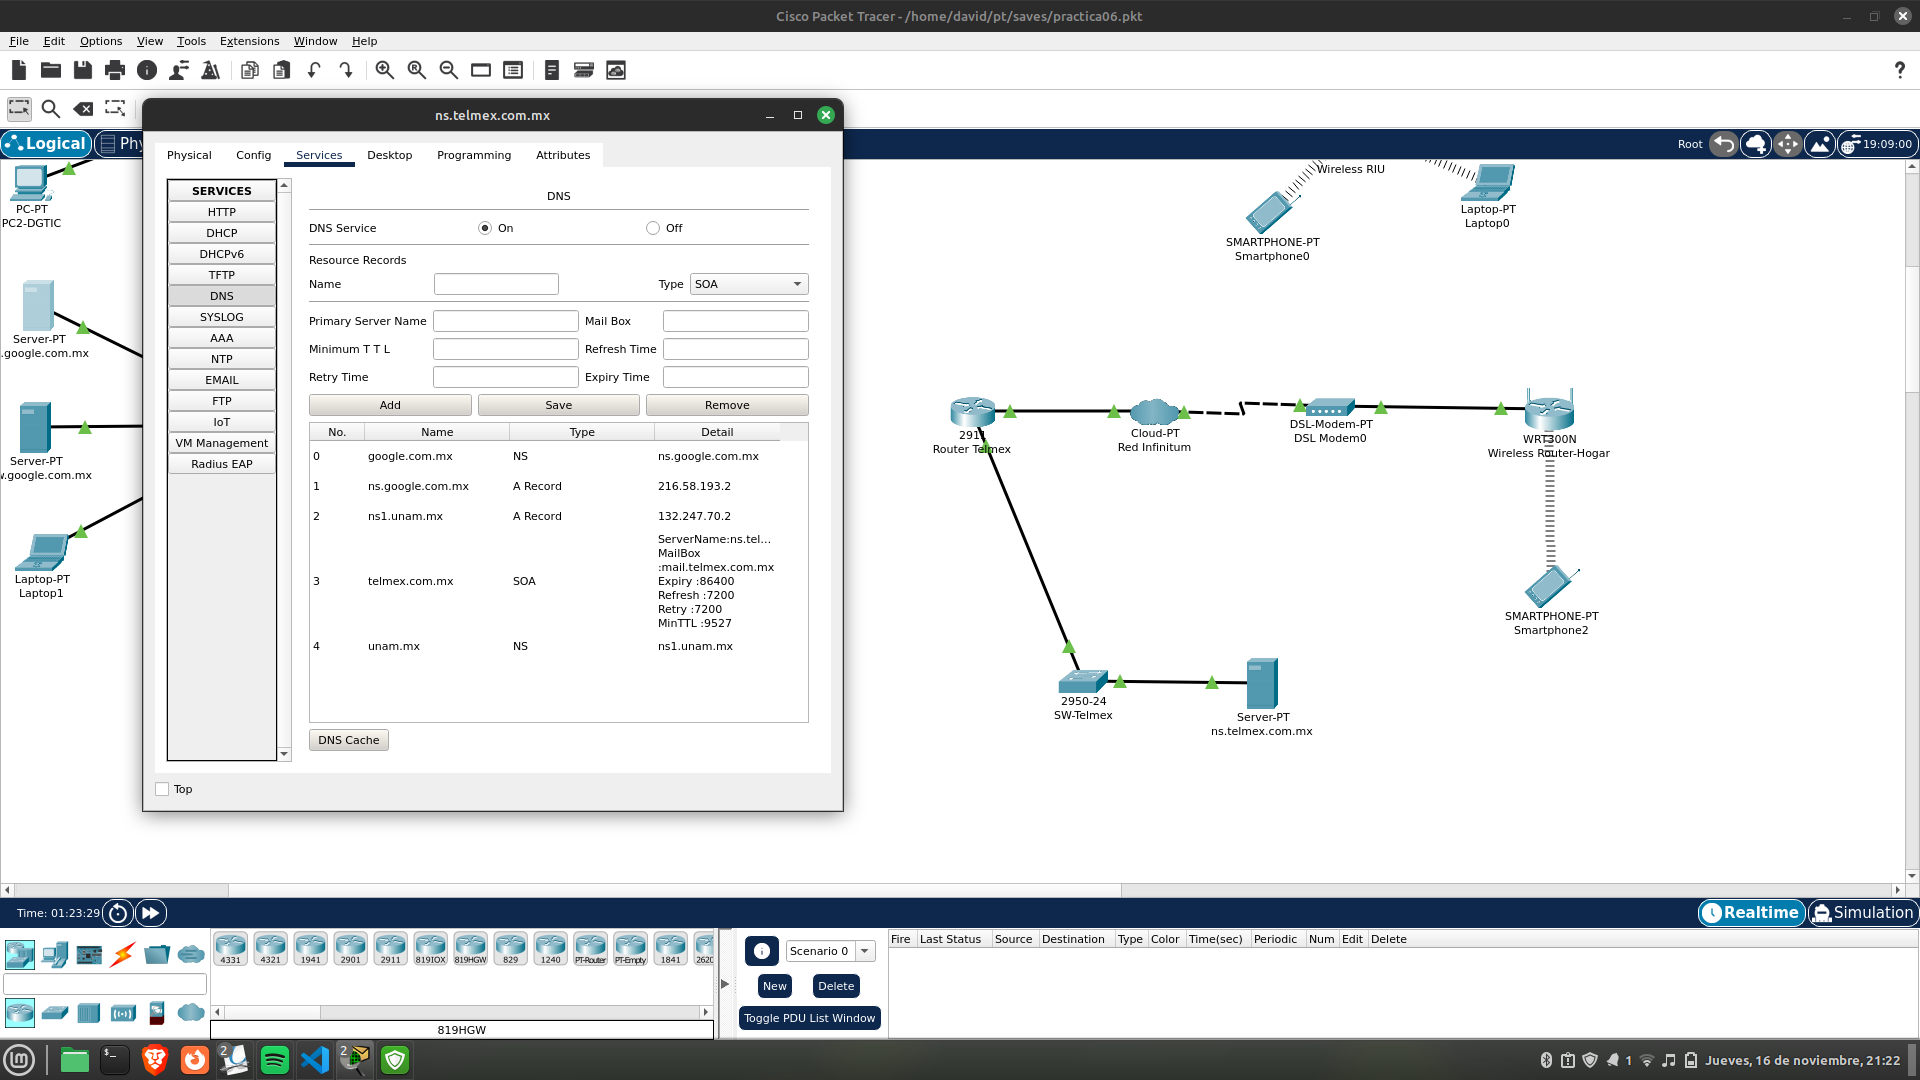
\includegraphics[width=12cm, height=8cm]{images/DNS Telmex-Infinitum.png}\\

TAmbien agregamos los siguientes registros al DNS-UNAM:

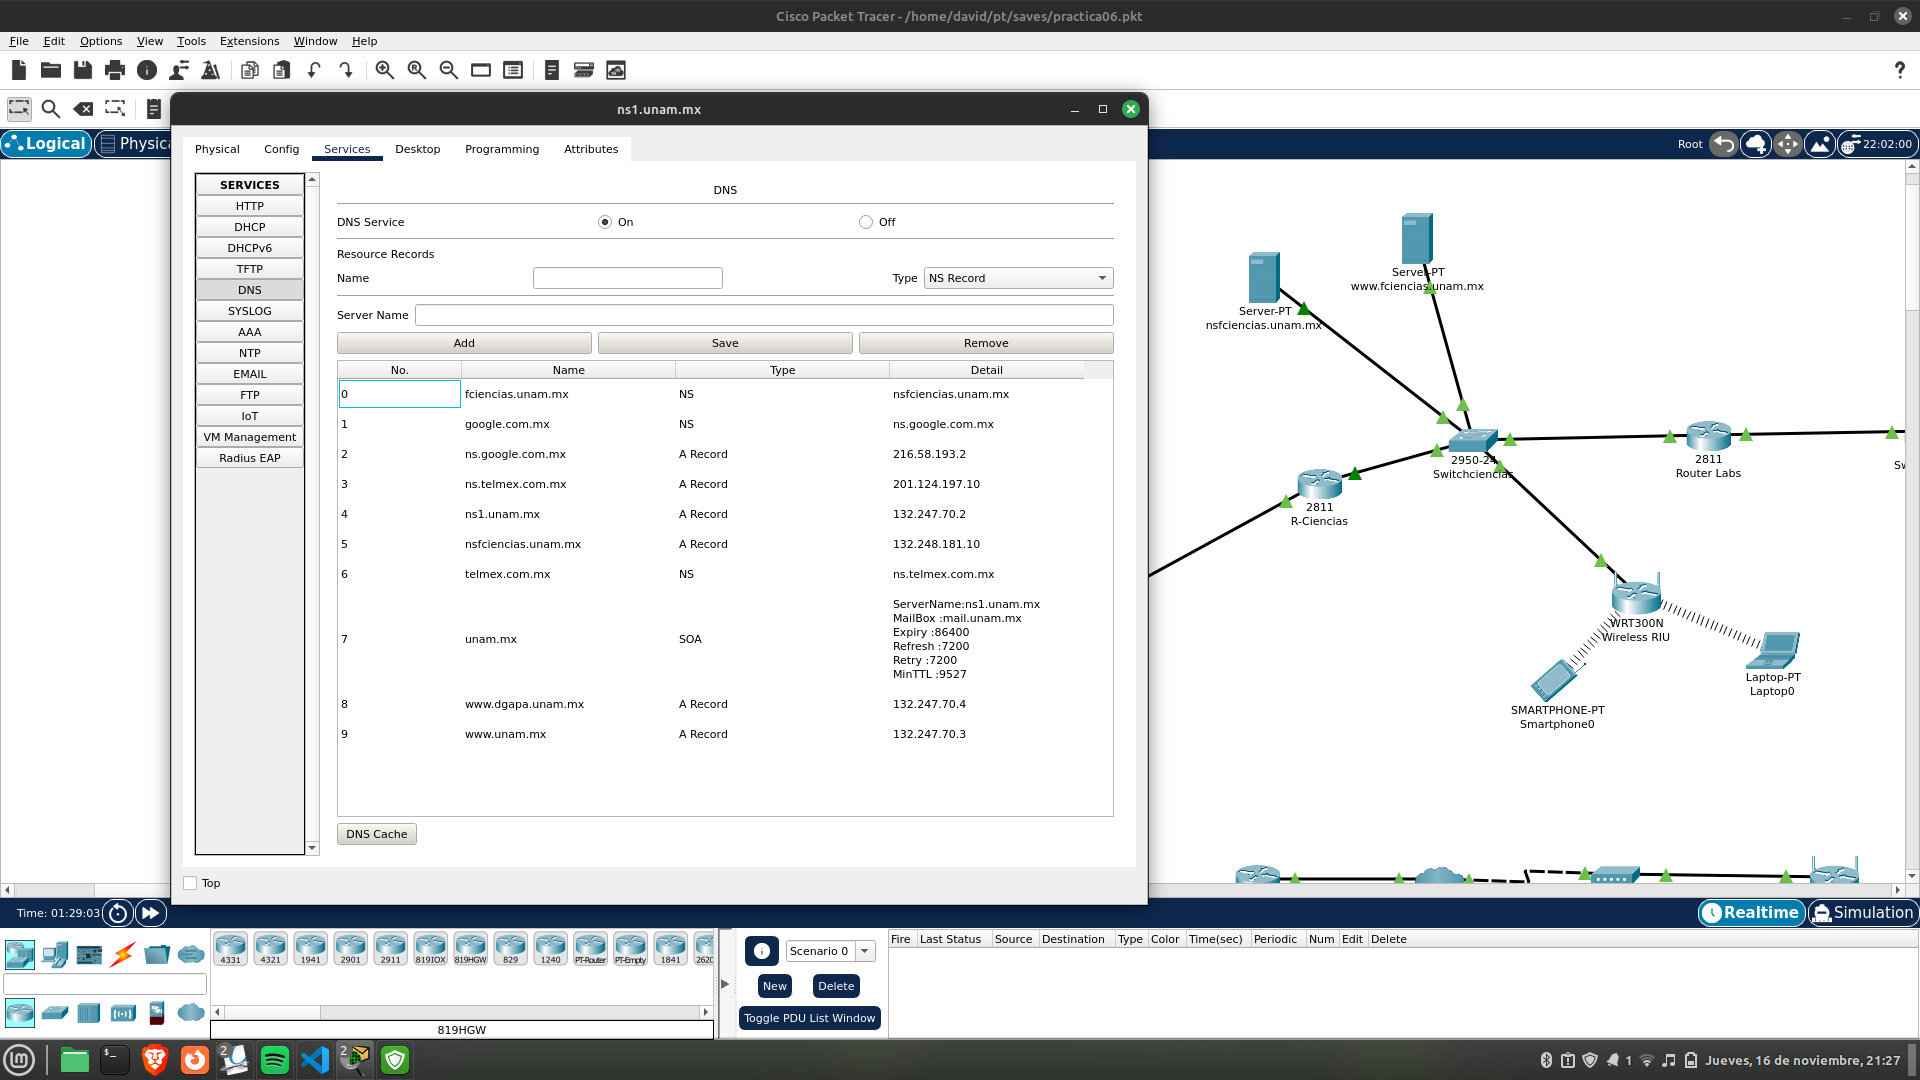
\includegraphics[width=12cm, height=8cm]{images/dns unam.png}\\

Y en el DNS-FCIENCIAS:\\

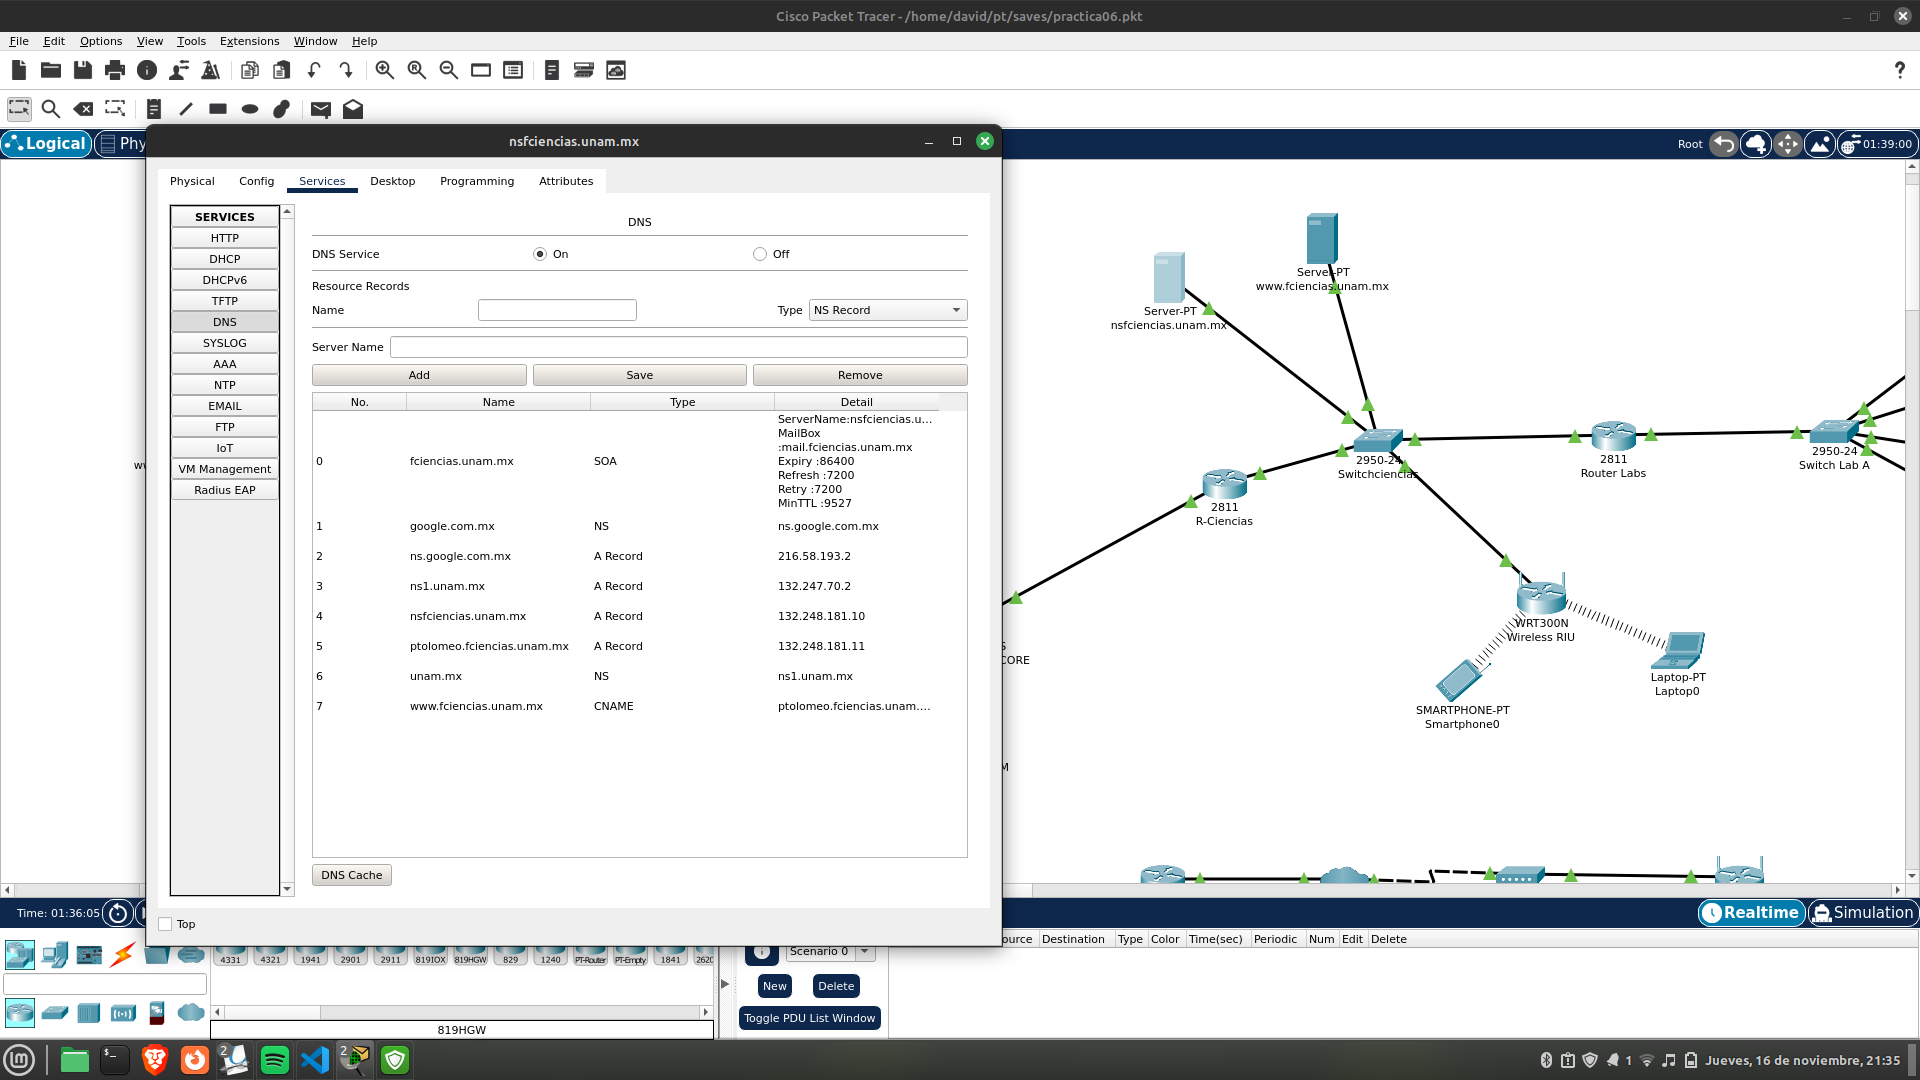
\includegraphics[width=12cm, height=8cm]{images/DNSCIENDIAS.png}\\

\textbf{Configuración de los Router UNAM, Google y Telmex:}\\

Agregamos a las 3 dispositivos una interfaz de red de tipo HWIC-2T.\\

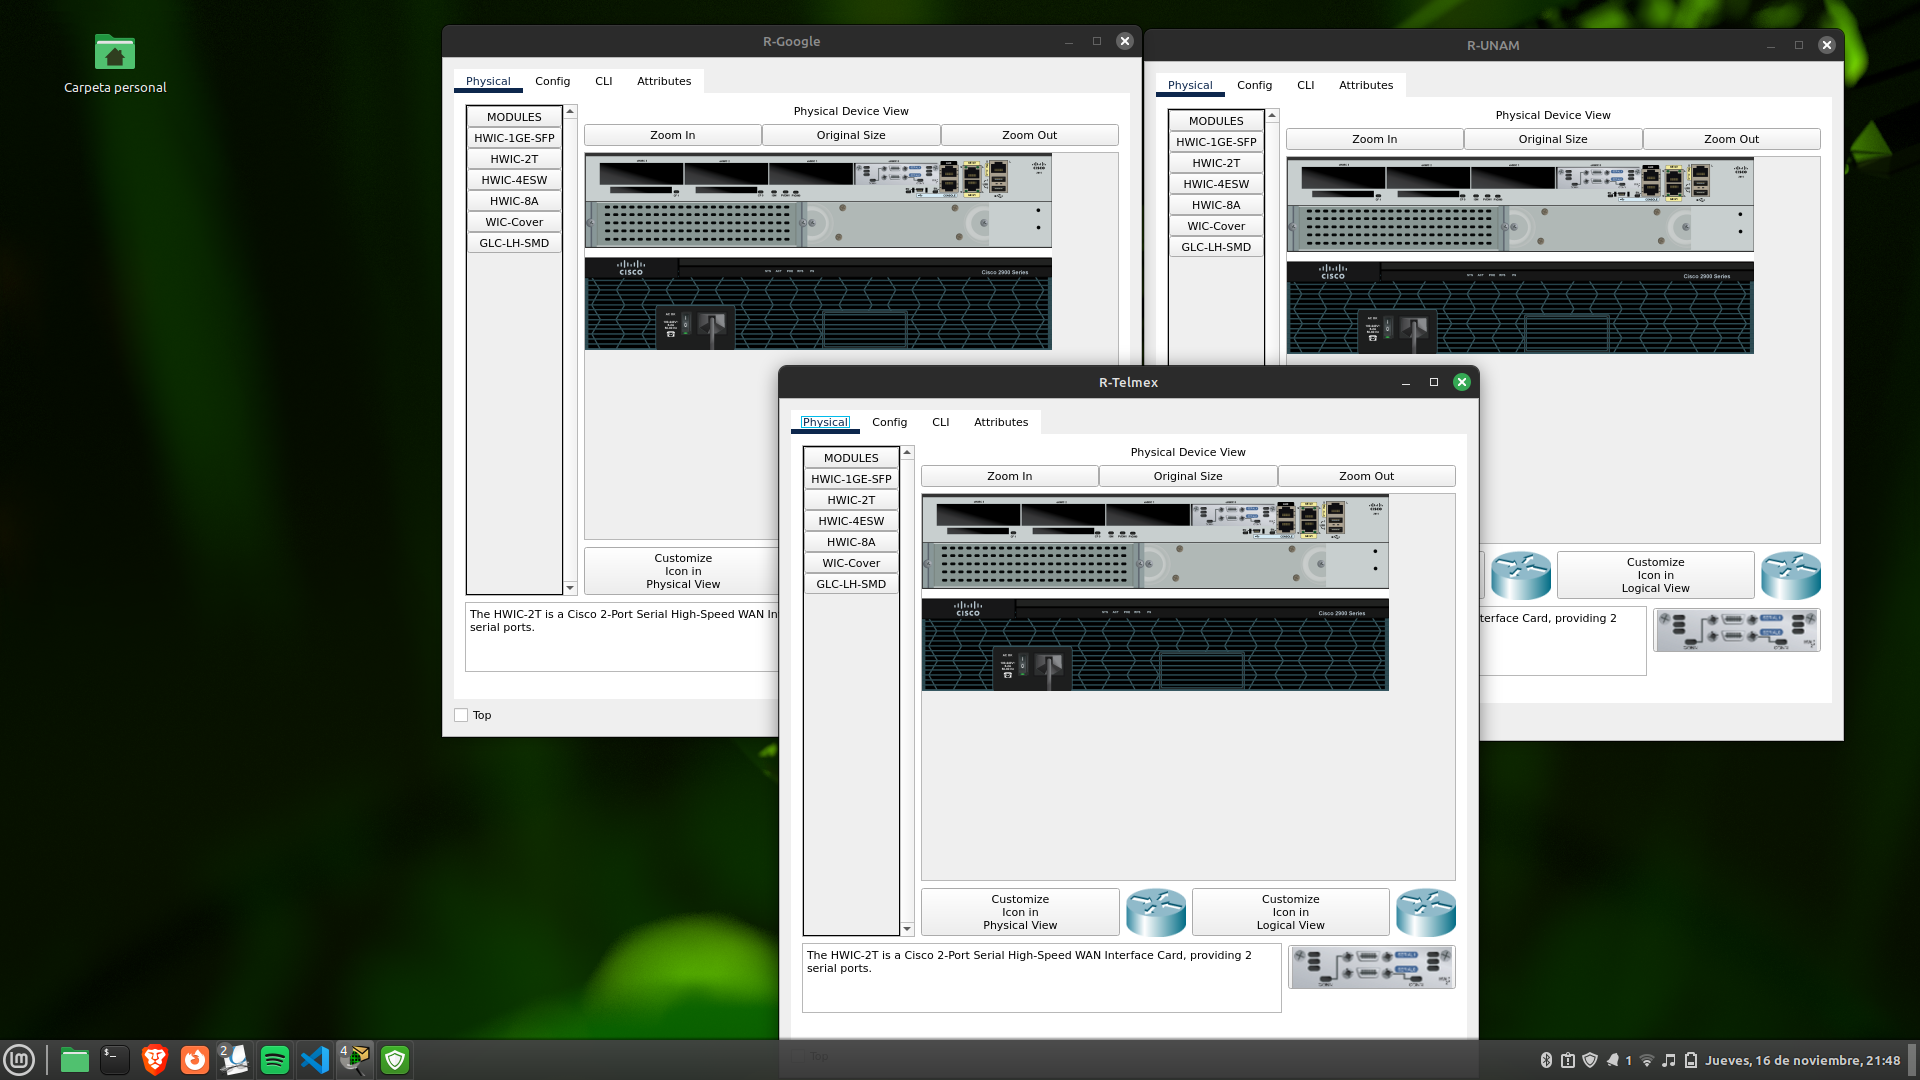
\includegraphics[width=12cm, height=8cm]{images/fisico de ruters.png}\\

Ahora configuramos los ruters como lo muestra la tabla del pdf de la Practica.\\

Para el Router-Unam:\\

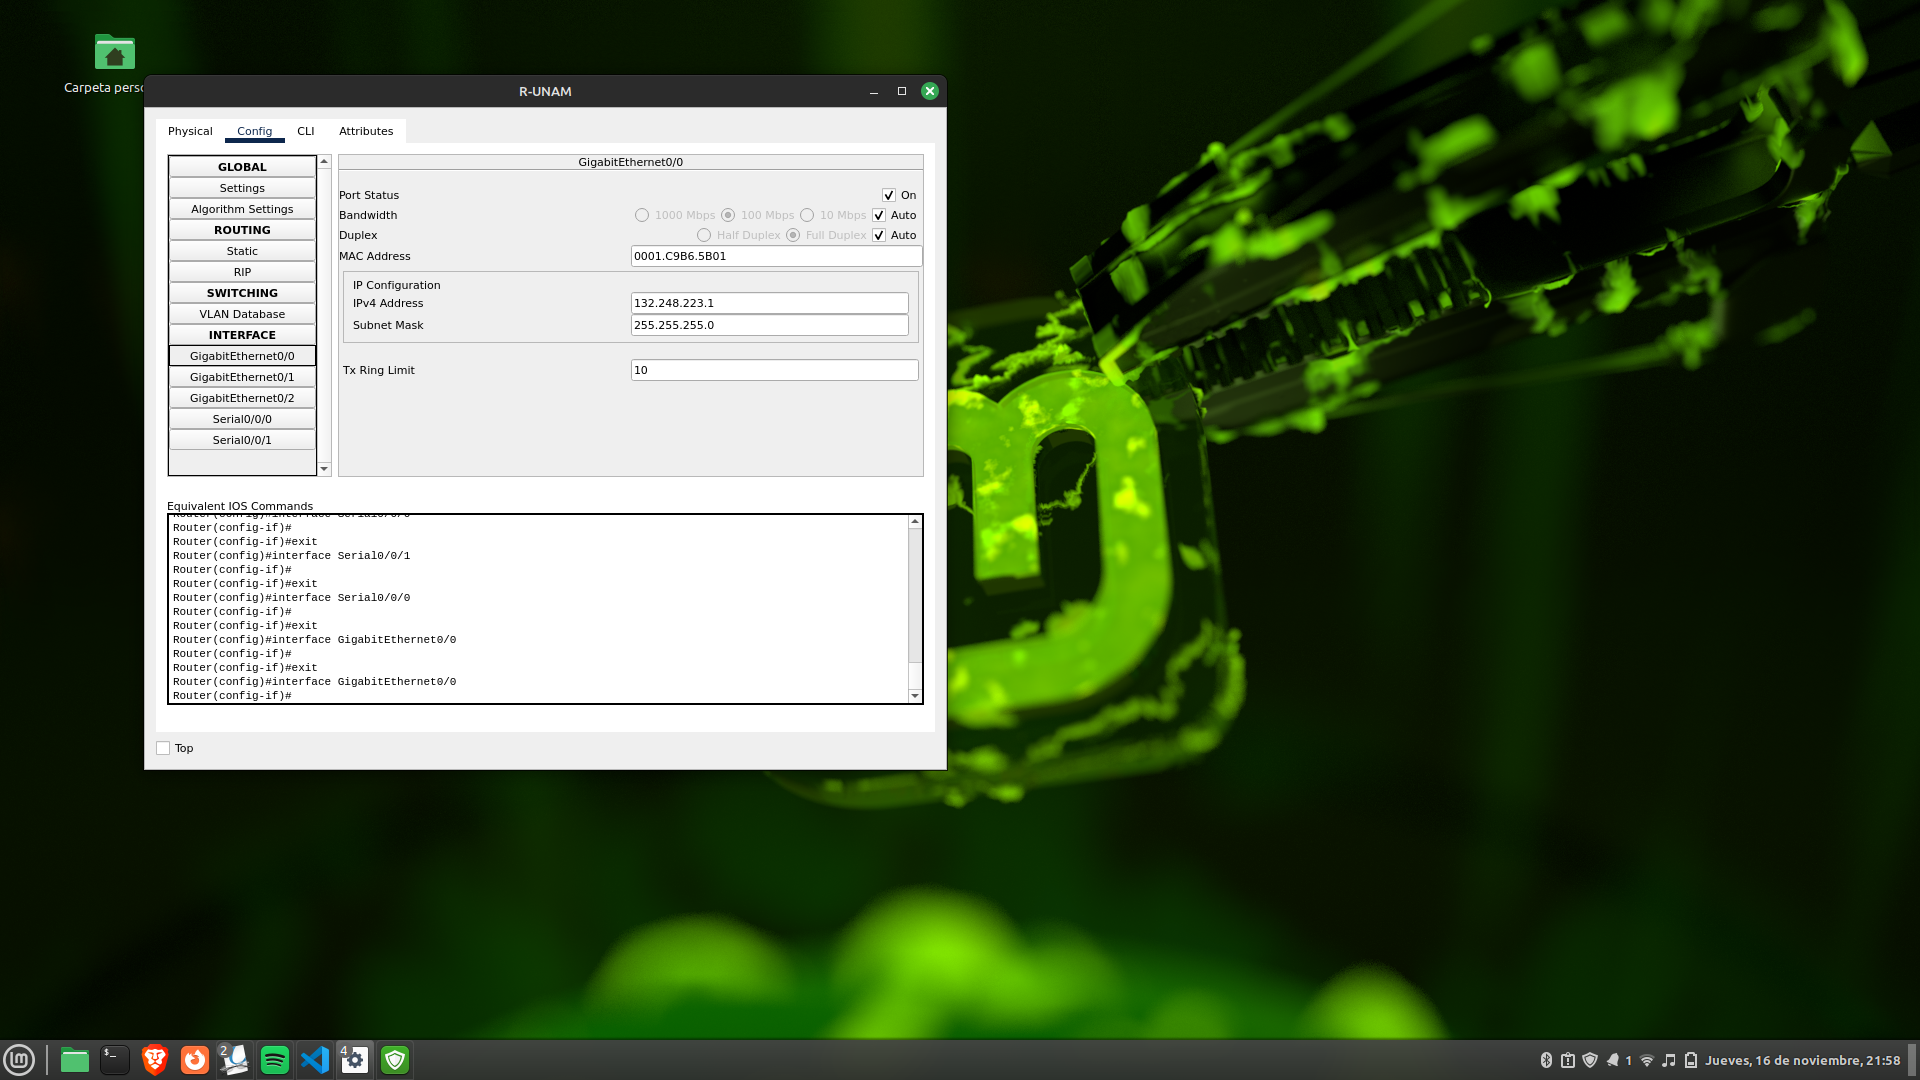
\includegraphics[width=12cm, height=8cm]{images/runam confi.png}\\

Para el Router-Google:\\

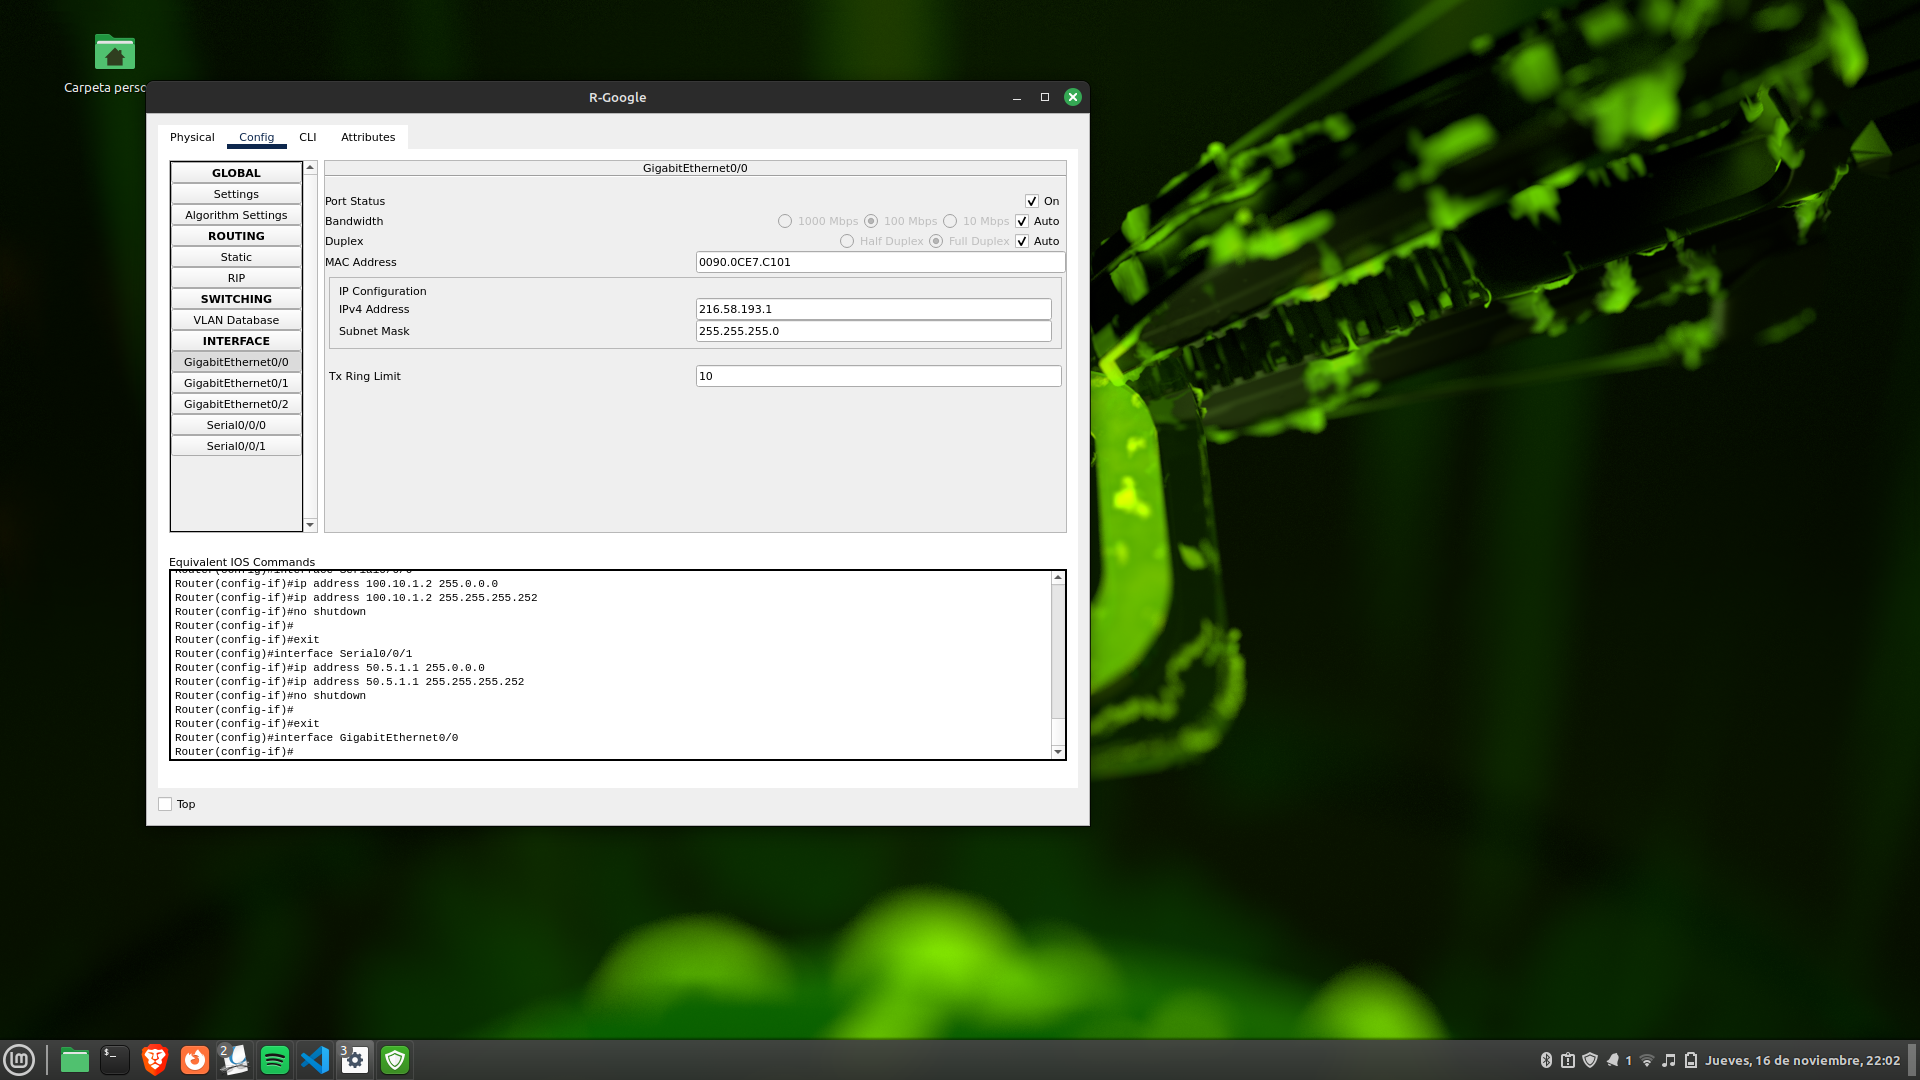
\includegraphics[width=12cm, height=8cm]{images/ruouter googlee.png}\\

Para el Router-Telmex:\\

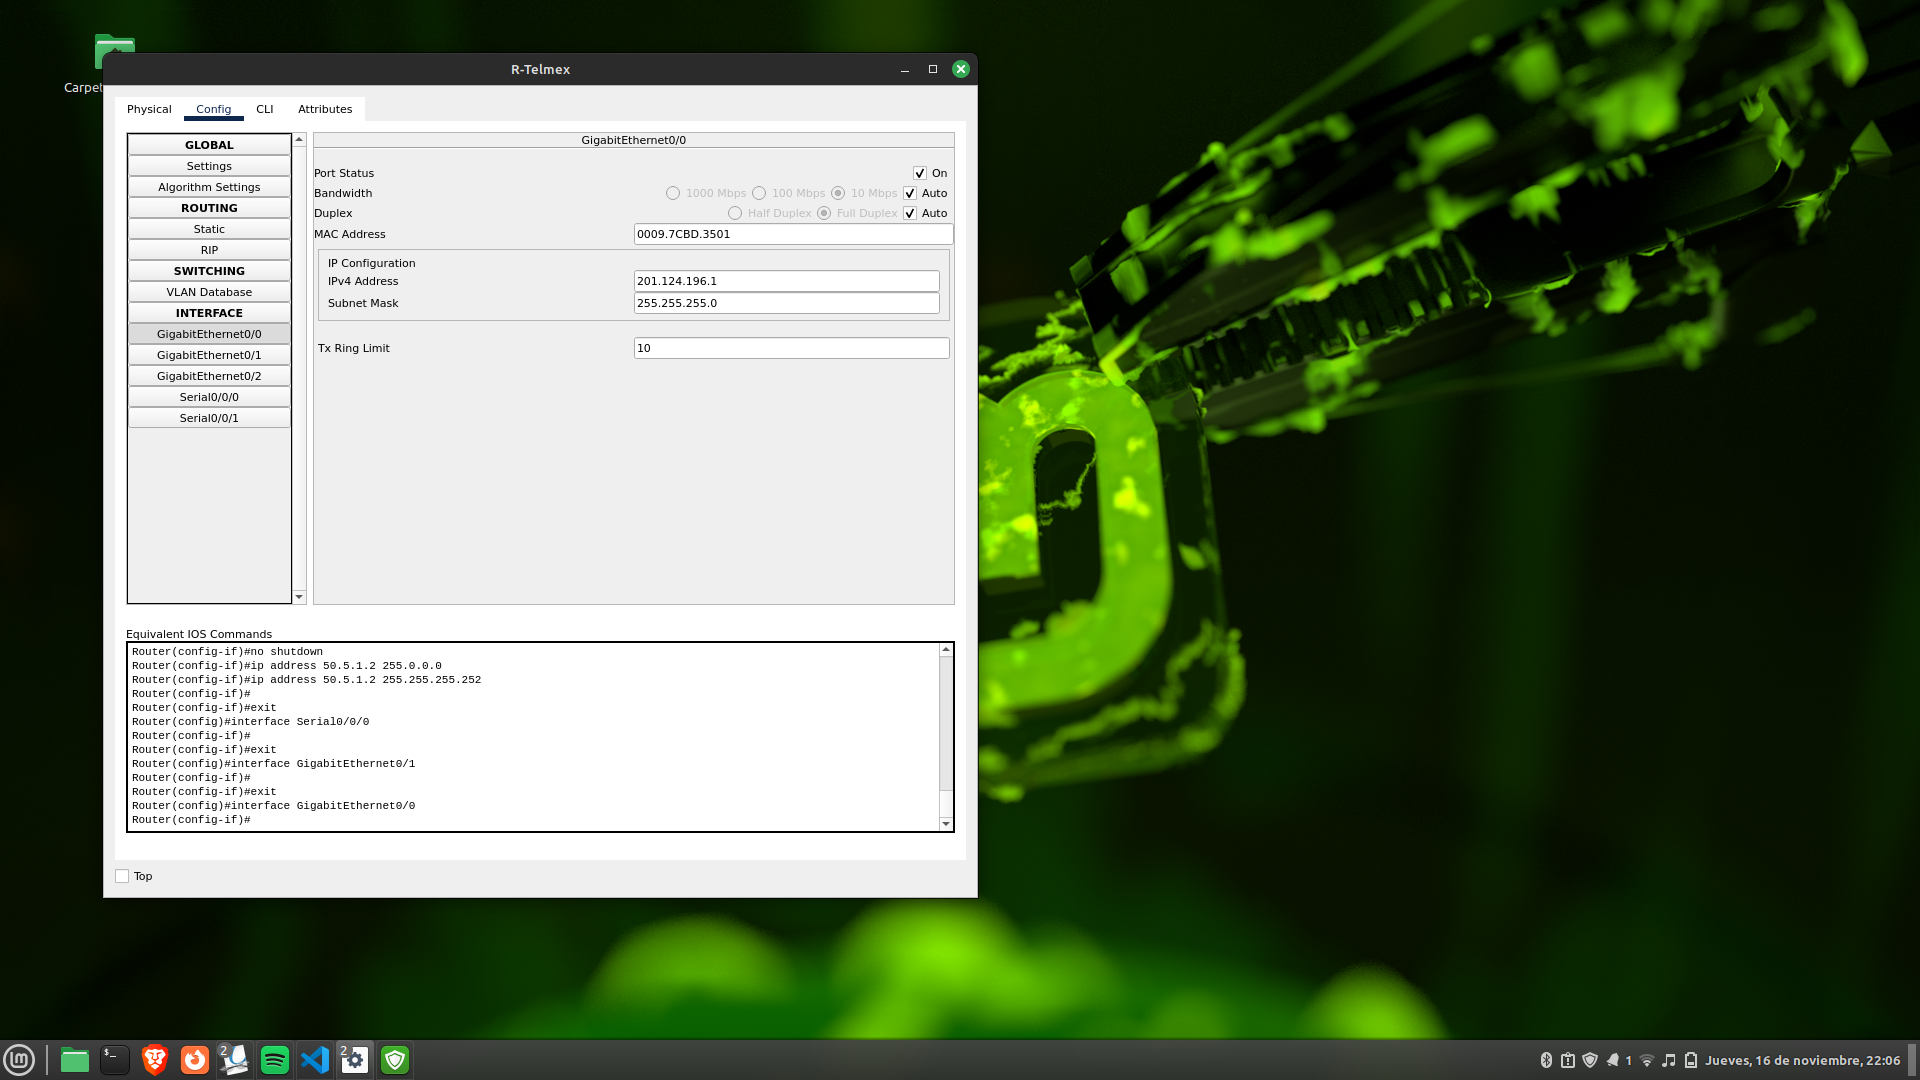
\includegraphics[width=12cm, height=8cm]{images/R-TELMEX.png}\\

Ahora conectamos los cables correspondientes con las conexiones, ya sea DCE o DTE de acuerdo a la tabla.\\

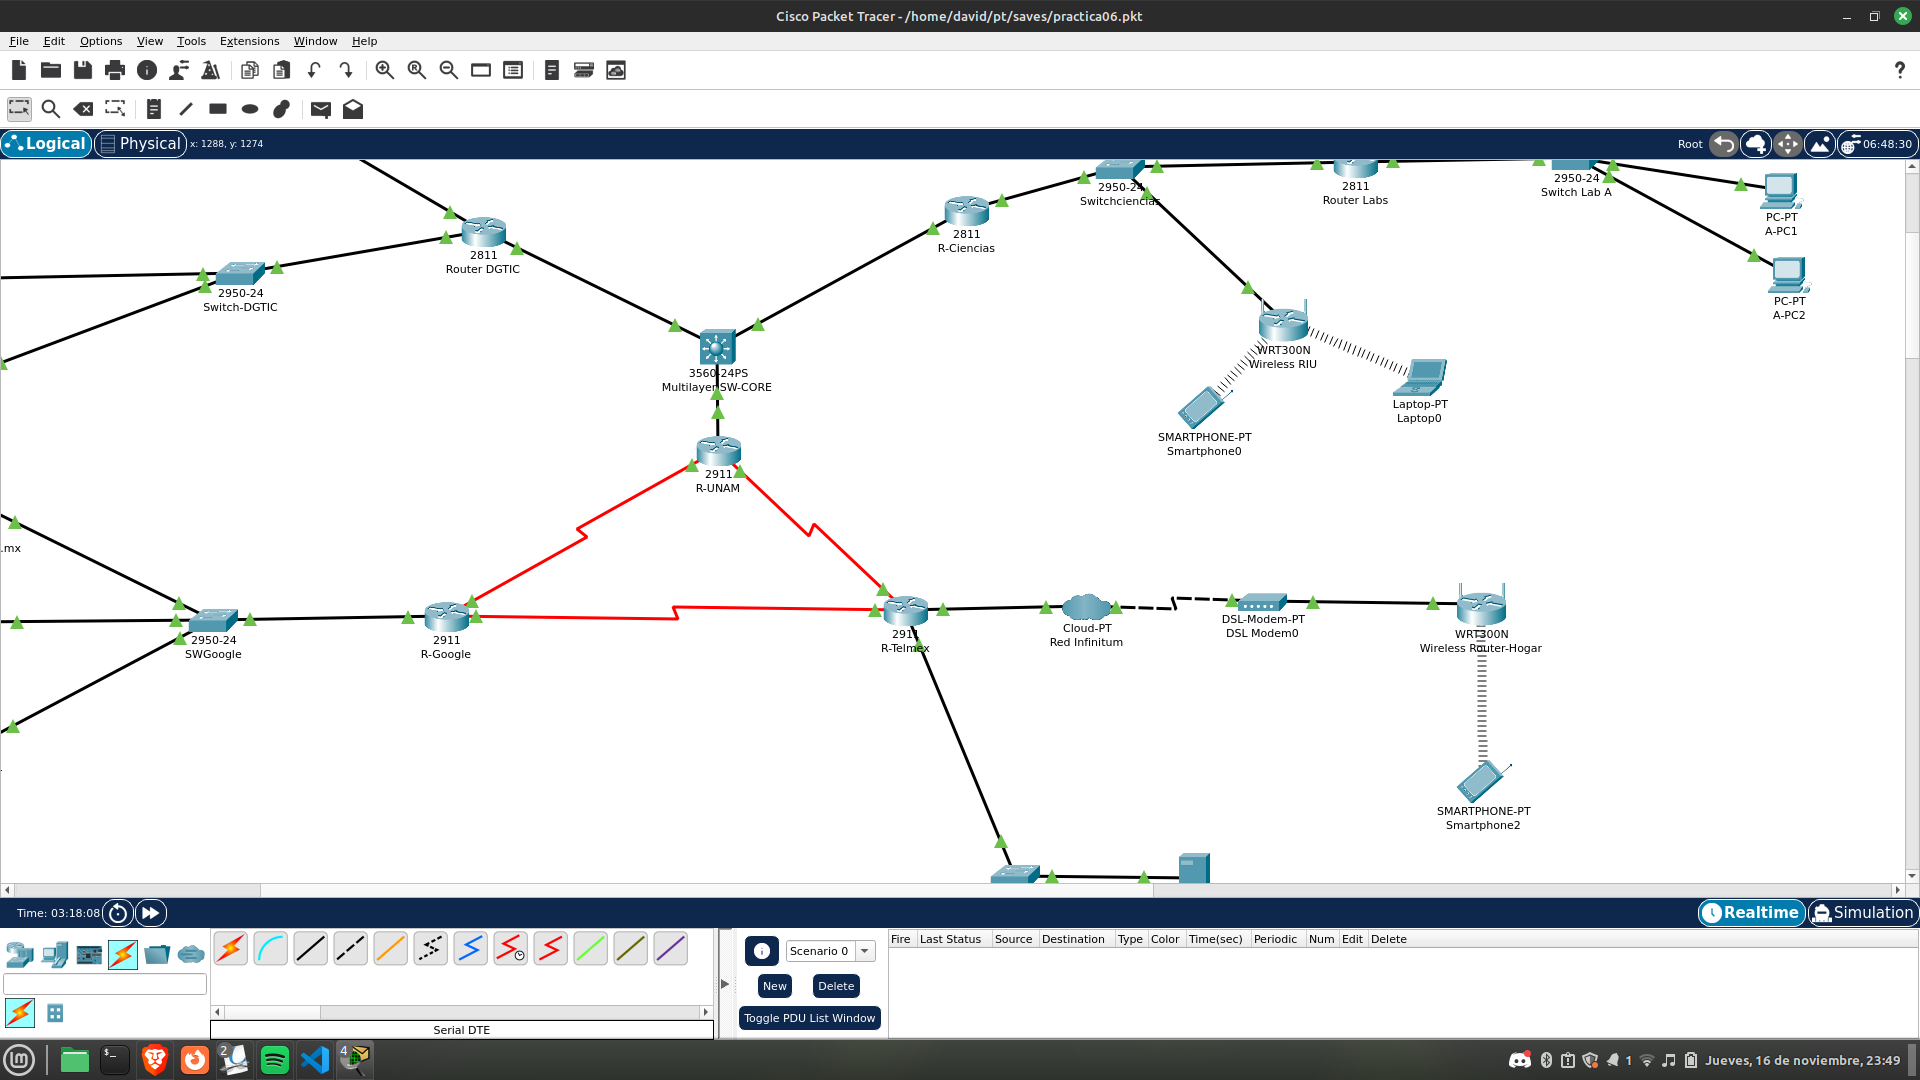
\includegraphics[width=12cm, height=8cm]{images/rojos.png}\\

Ahora seguiremos con el ultimo paso: \textbf{Configuración de rutas dinámicas.}\\

solo agregamos las direcciones Ip correspondientes a nuestros routers:\\

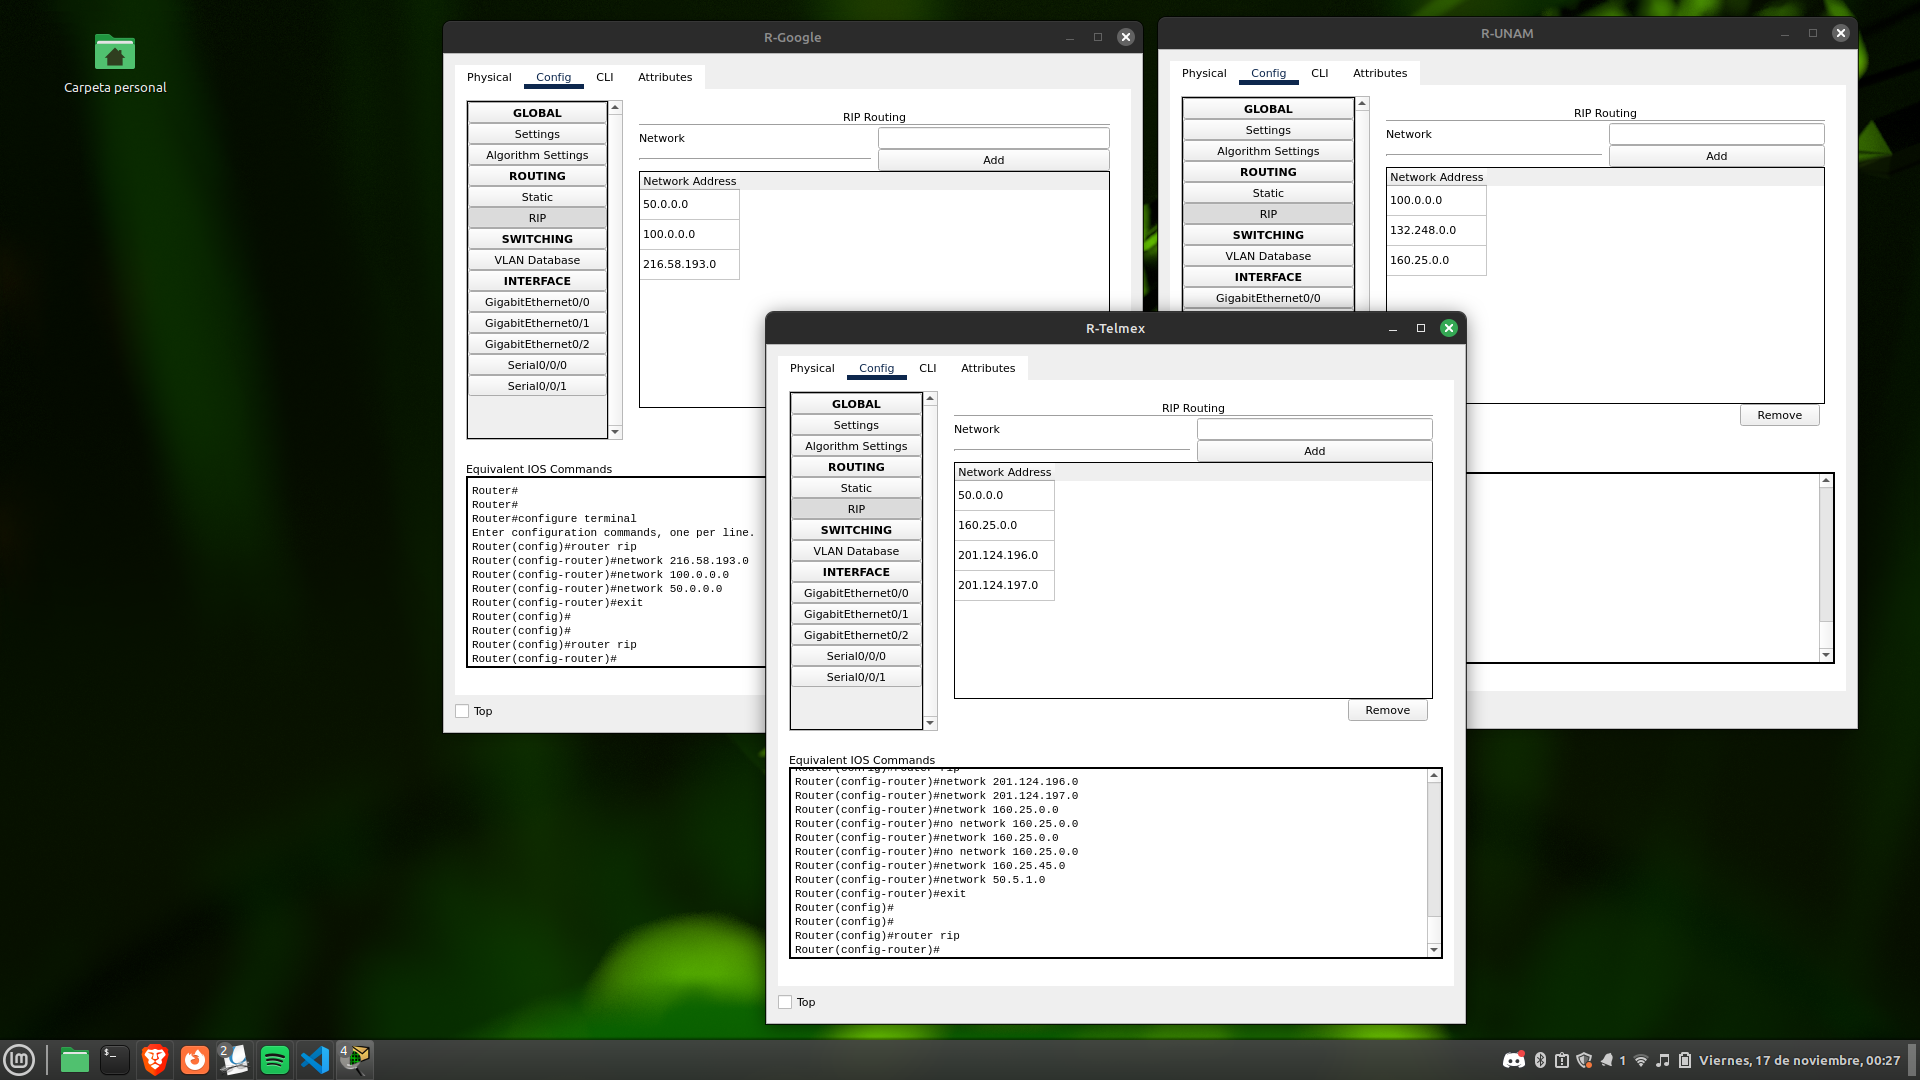
\includegraphics[width=12cm, height=8cm]{images/ip correspondienrs.png}\\

{\color{red} \subsection*{\textbf{Comprobar conexión}}}
\vspace{1em}

Para las pruebas estuve batallando demasiado con las configuraciones de los routers, en una simulación se veia que habia un problema en los routers, pero al final solo debia de configurar despues de conectar los cables de color rojo,
con base a ello ya se logró ingresar a las distintas paginas desde los distintos dispositivos.\\


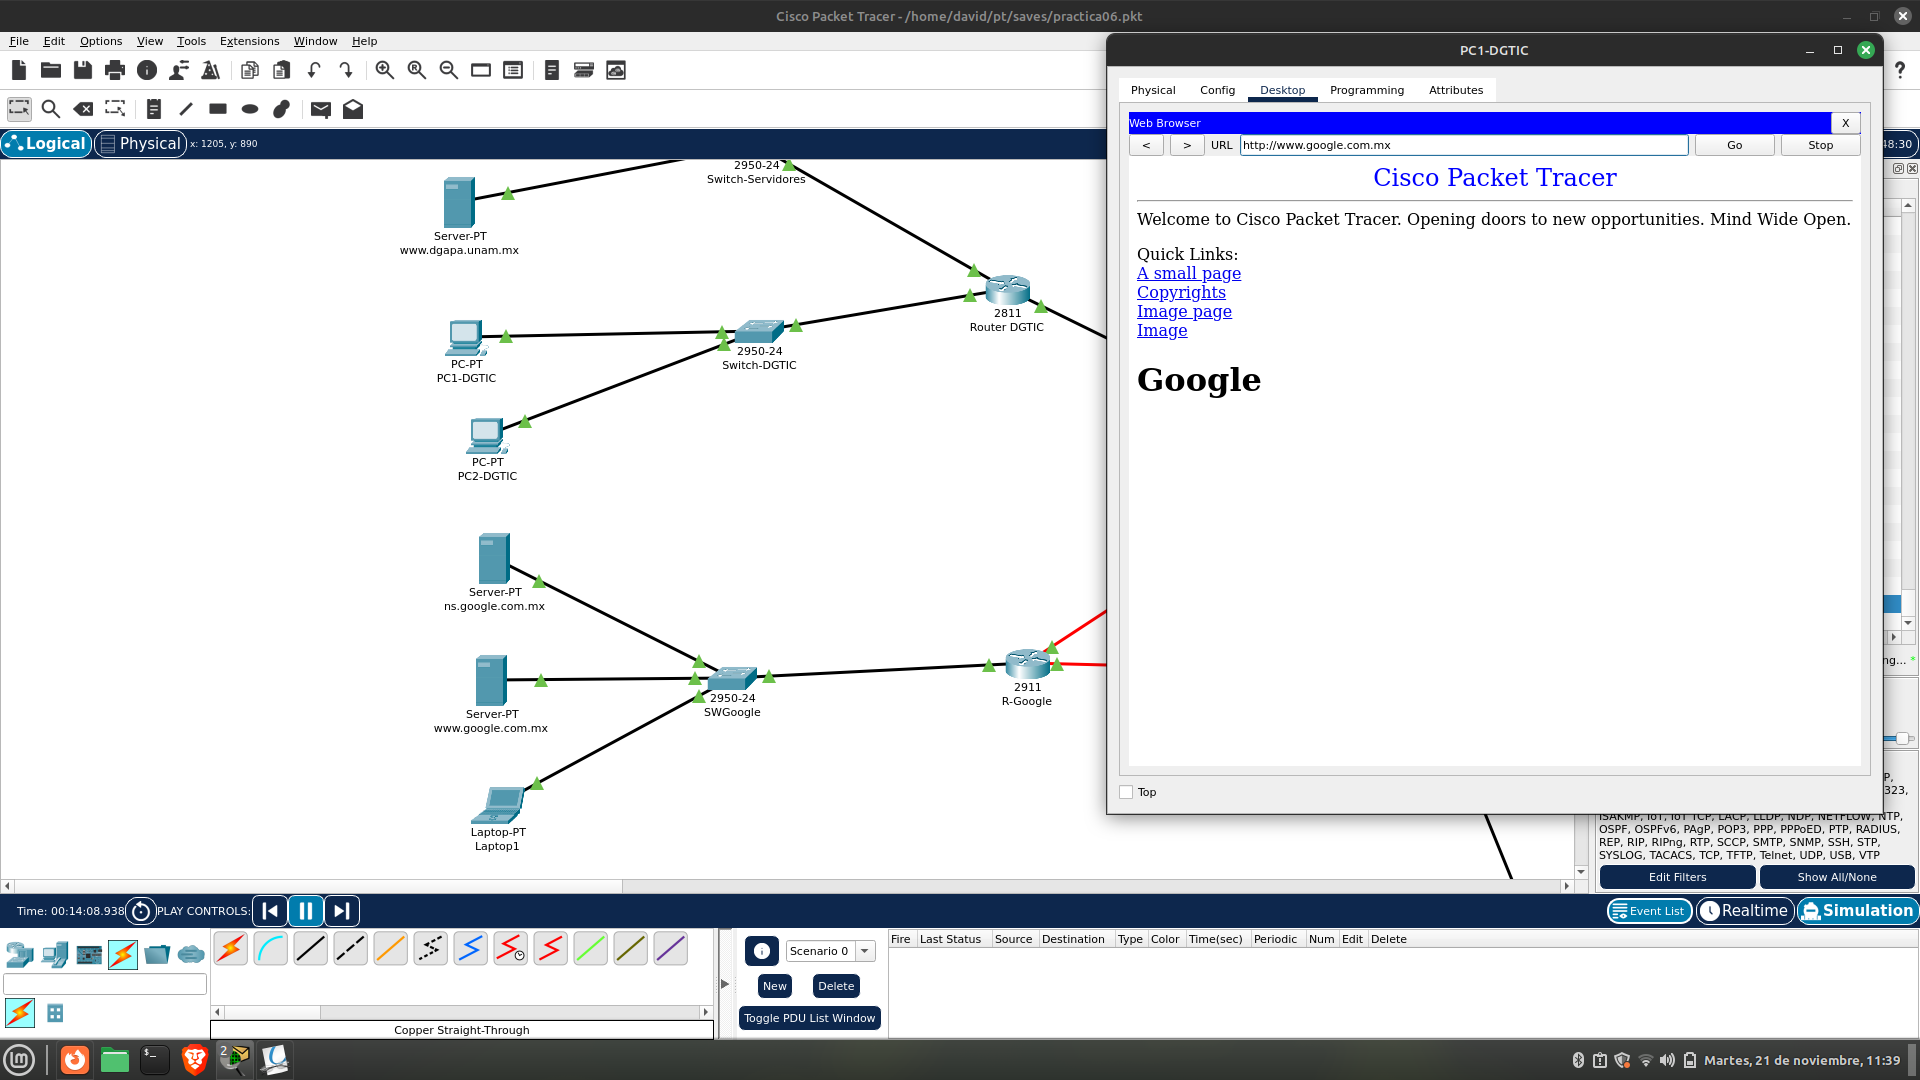
\includegraphics[width=12cm, height=8cm]{images/prueba1siiiiiiiii.png} PC1-DGTIC\\

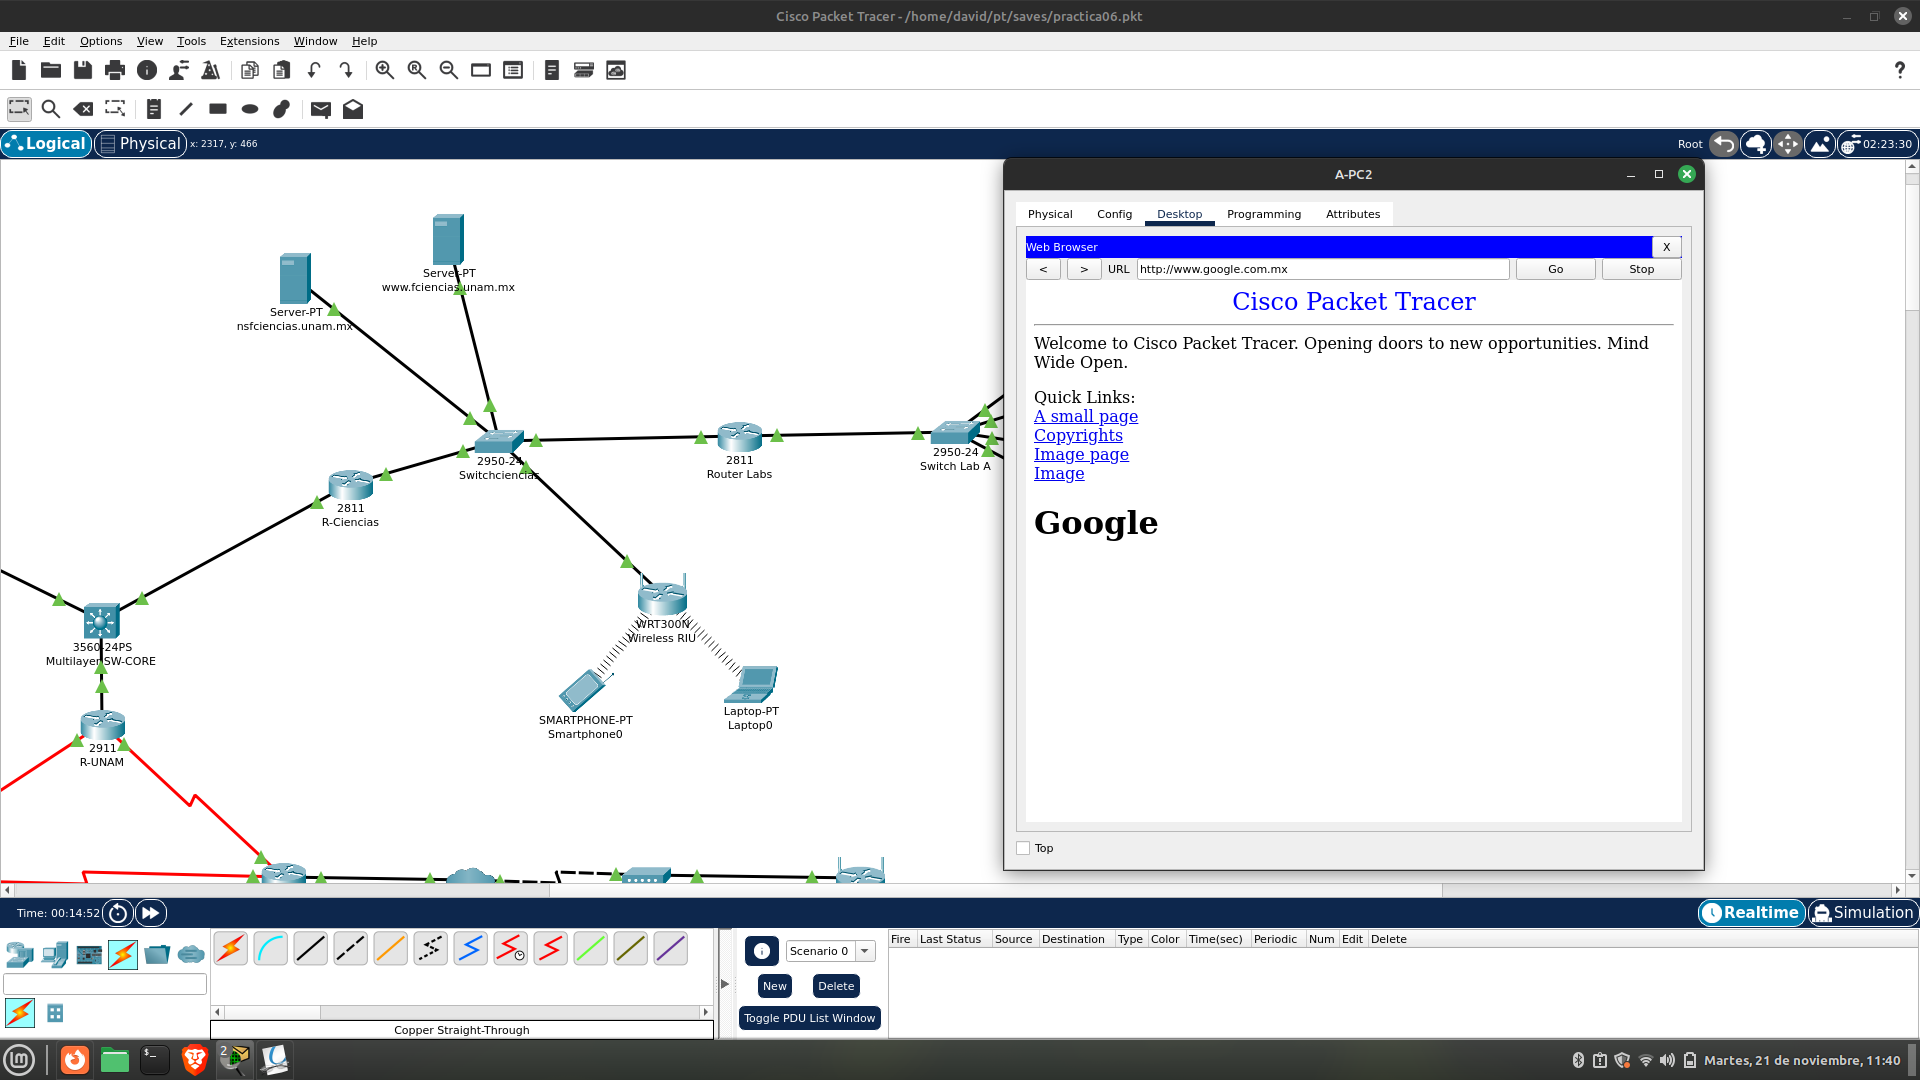
\includegraphics[width=12cm, height=8cm]{images/prueba 2 siiiiiii.png} A-PC2\\

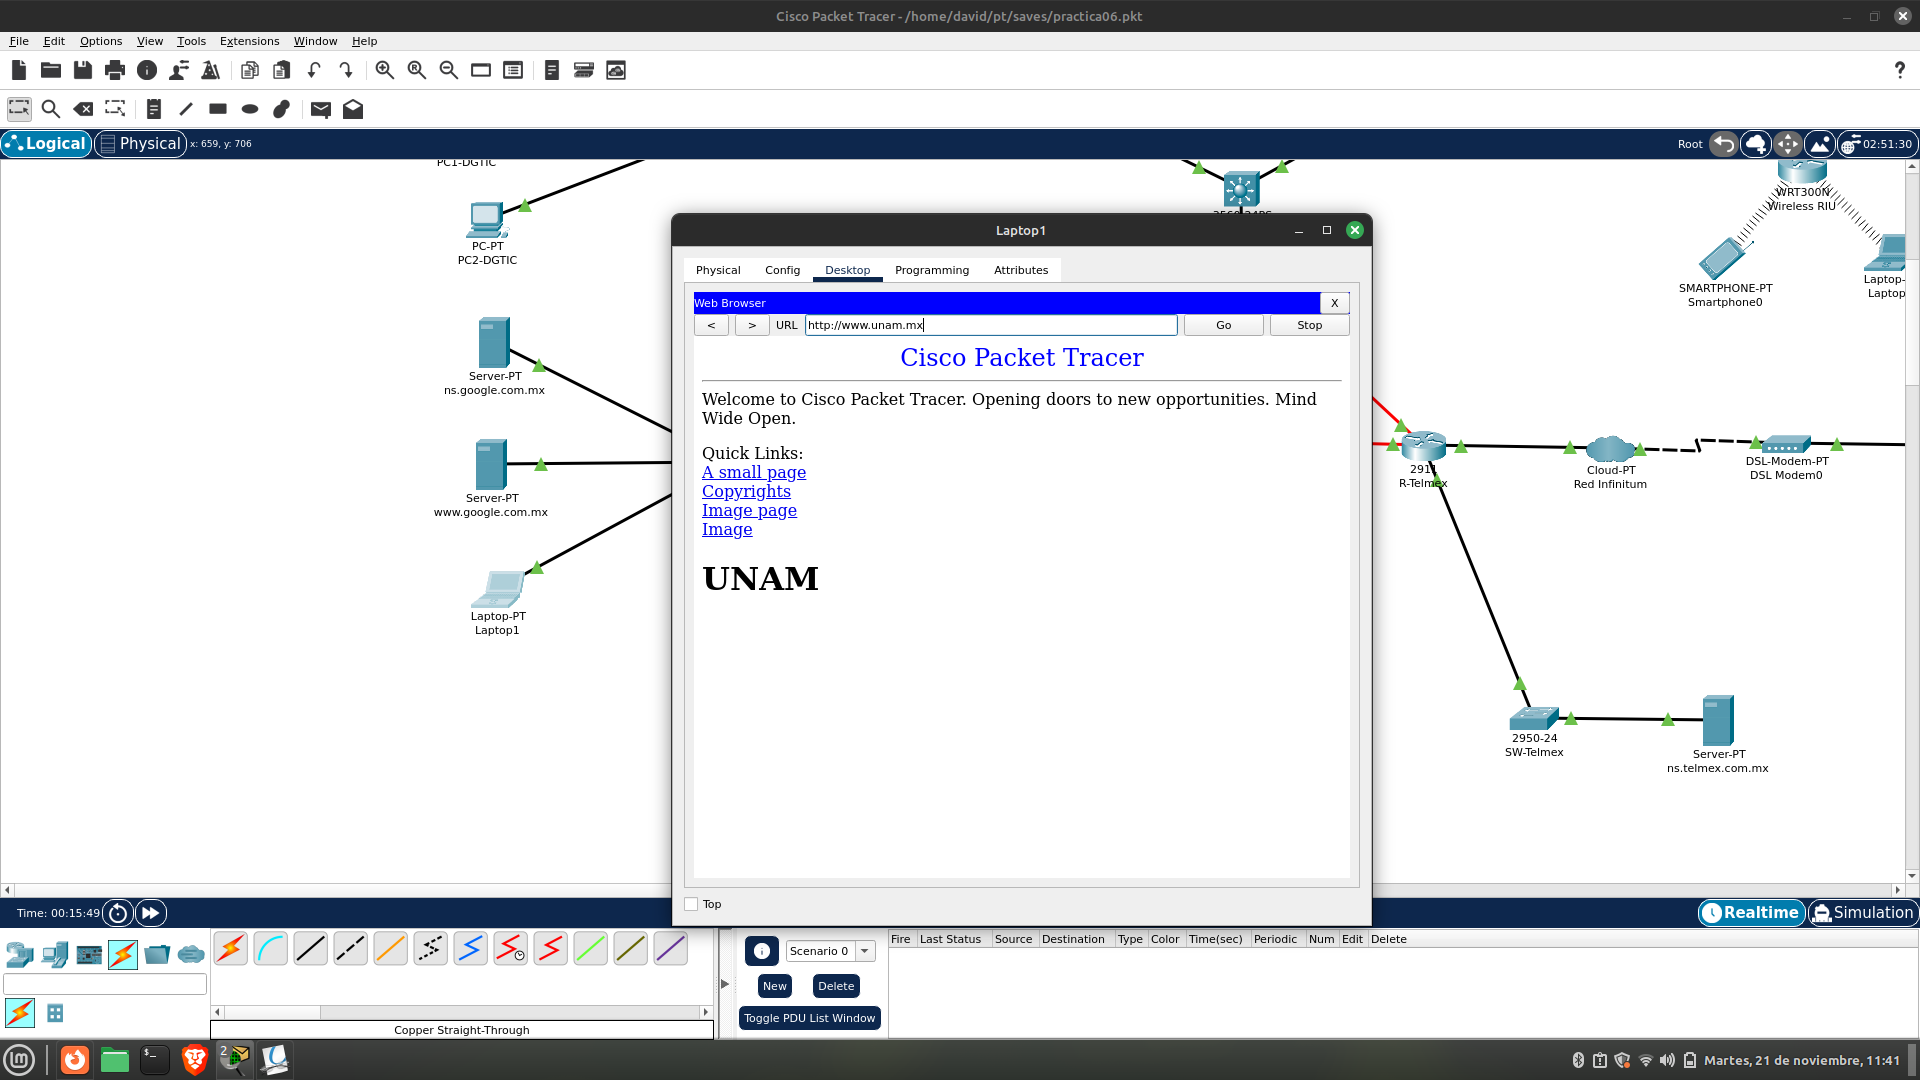
\includegraphics[width=12cm, height=8cm]{images/prueba 3 siiii.png} Laptop1 a www.unam.mx\\

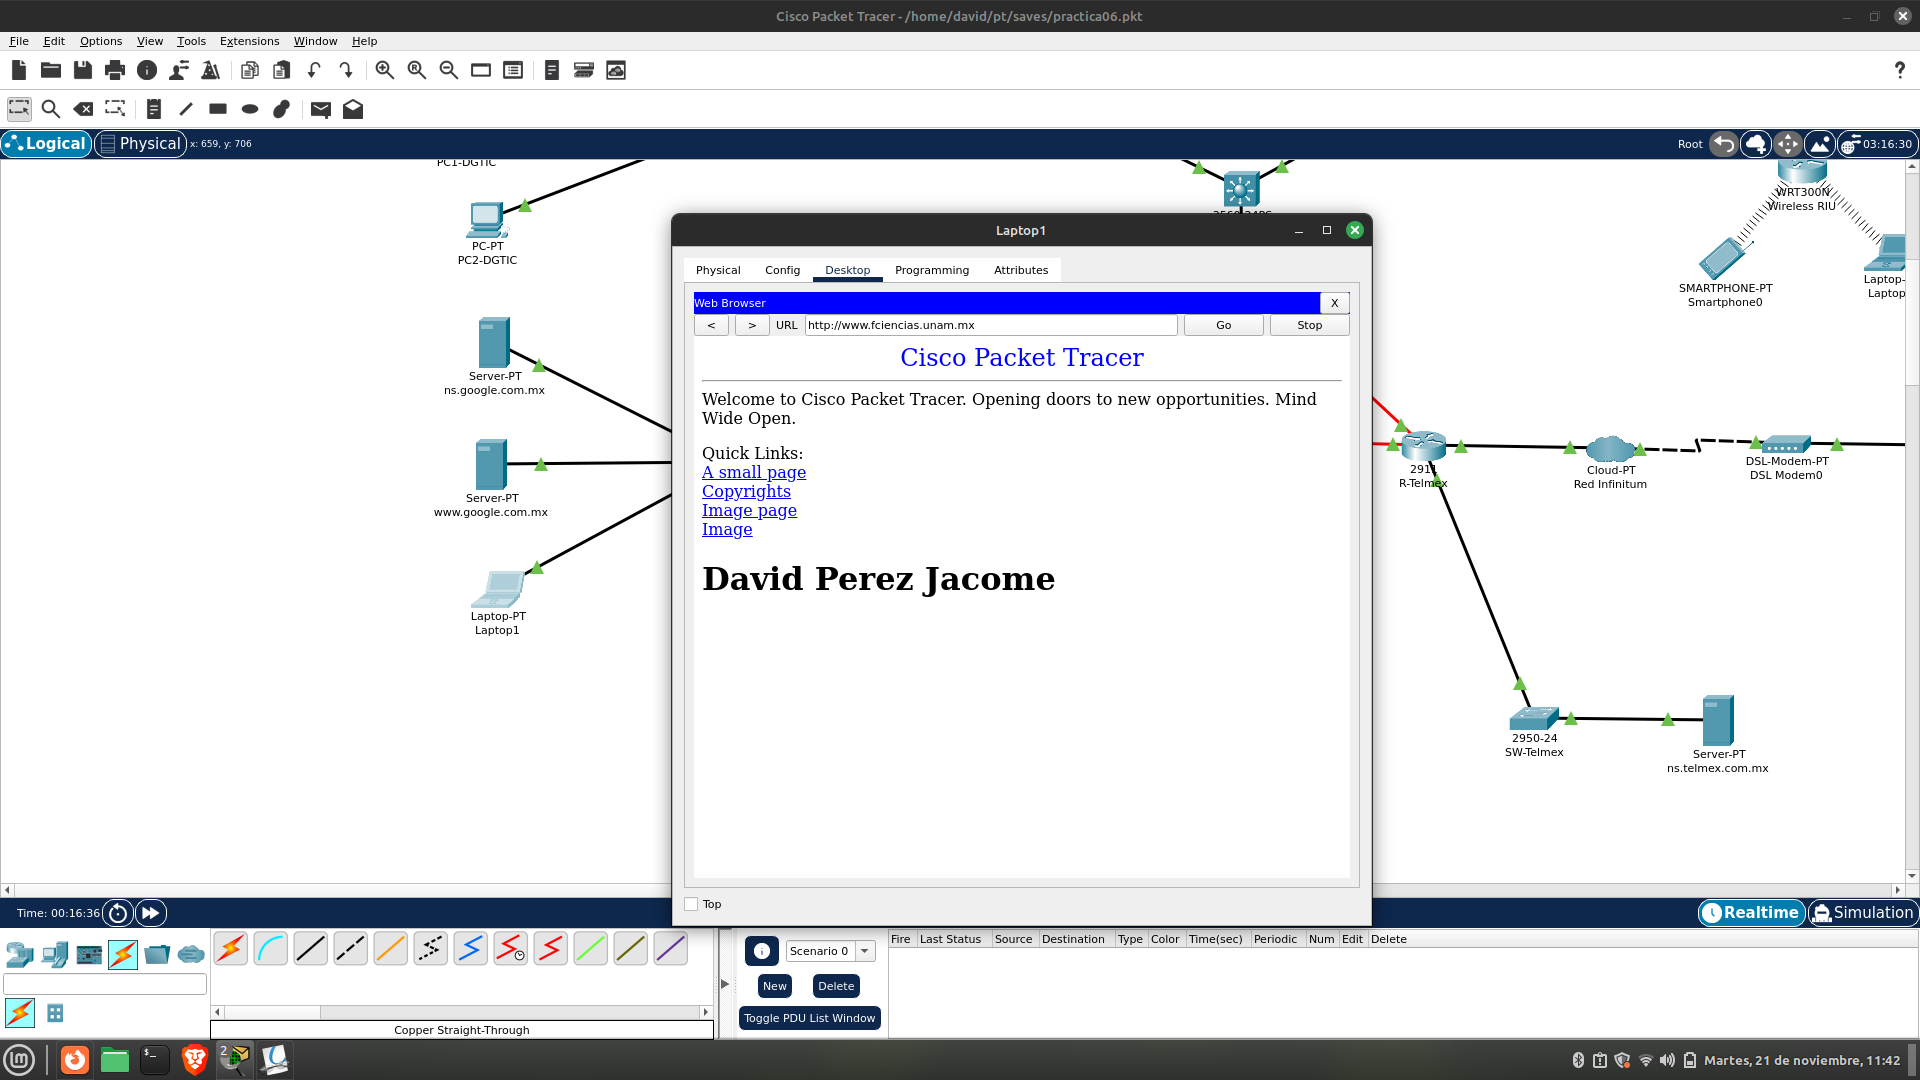
\includegraphics[width=12cm, height=8cm]{images/prueba 4 siiiiiiii.png} Laptop1 a www.fciencias.unam.mx\\

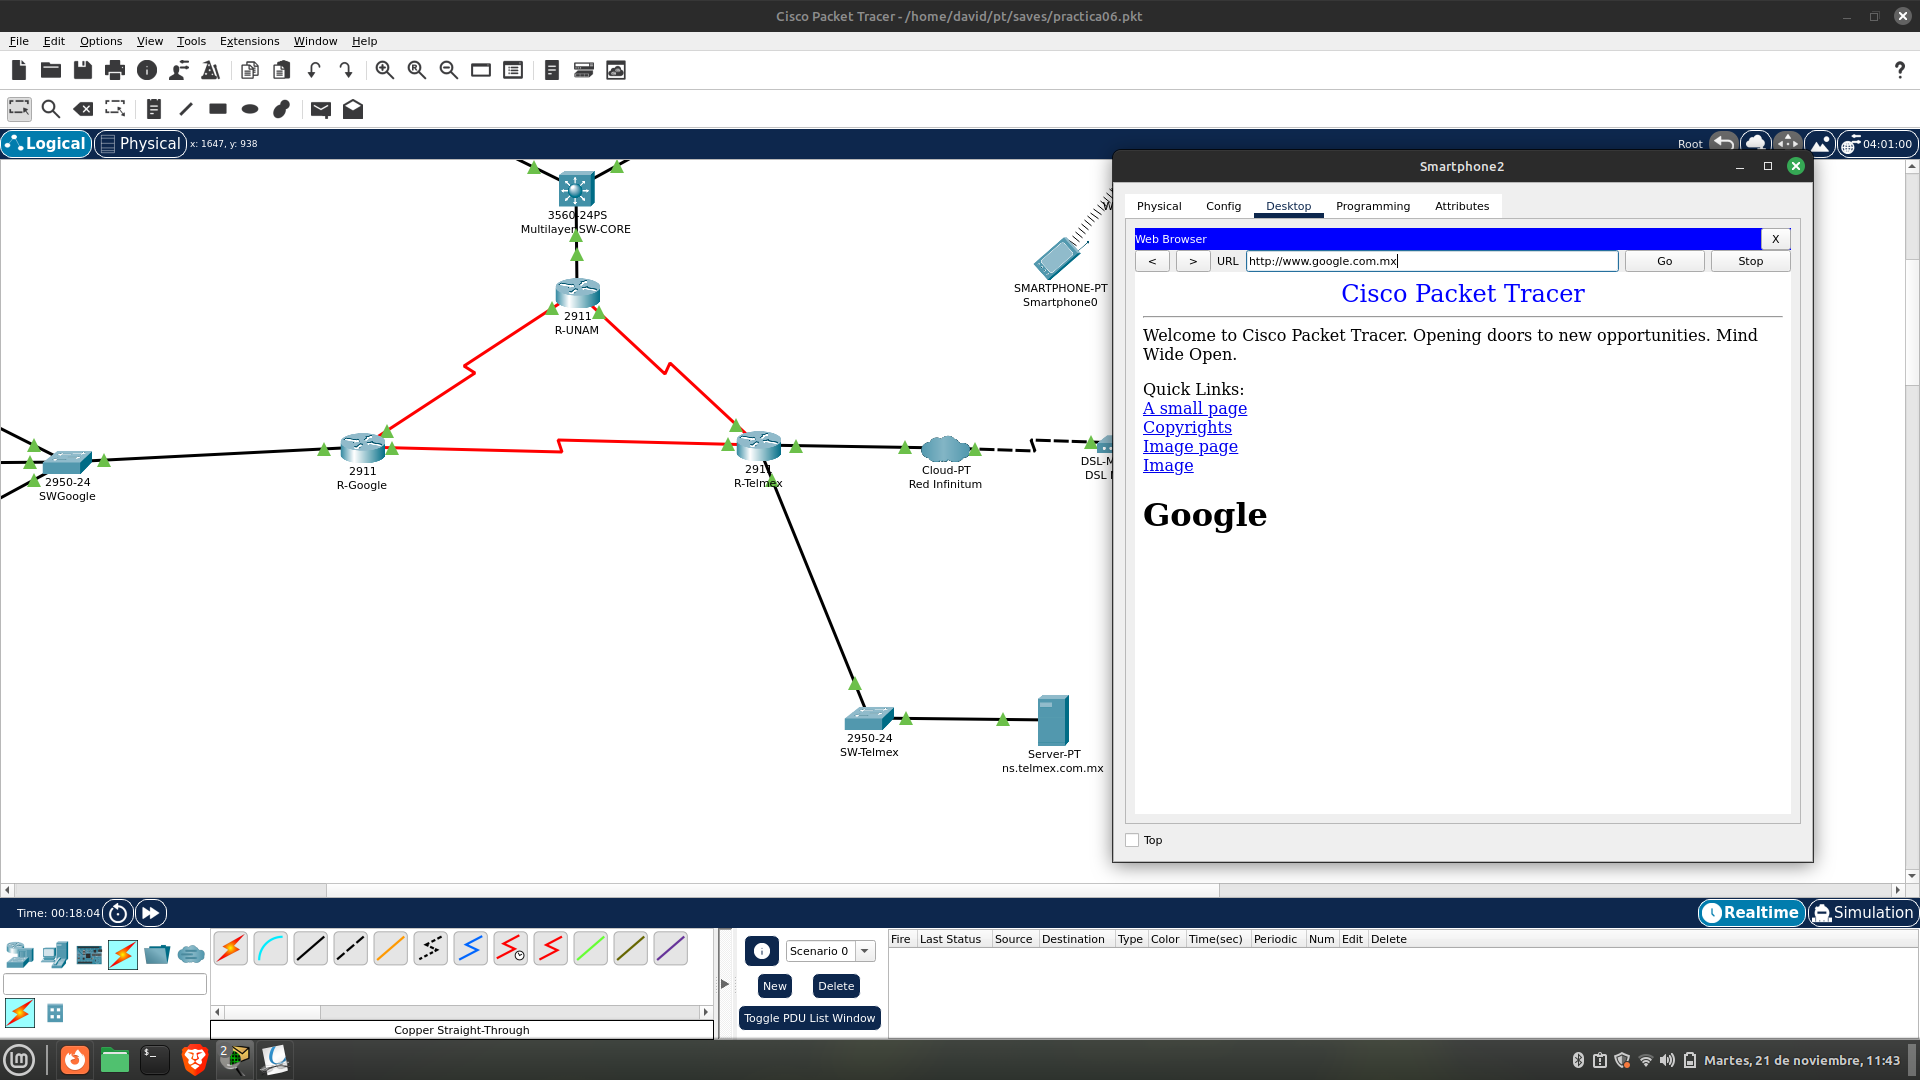
\includegraphics[width=12cm, height=8cm]{images/prueba 4-5 siiiiii.png} Smartphone2 a  www.google.com\\

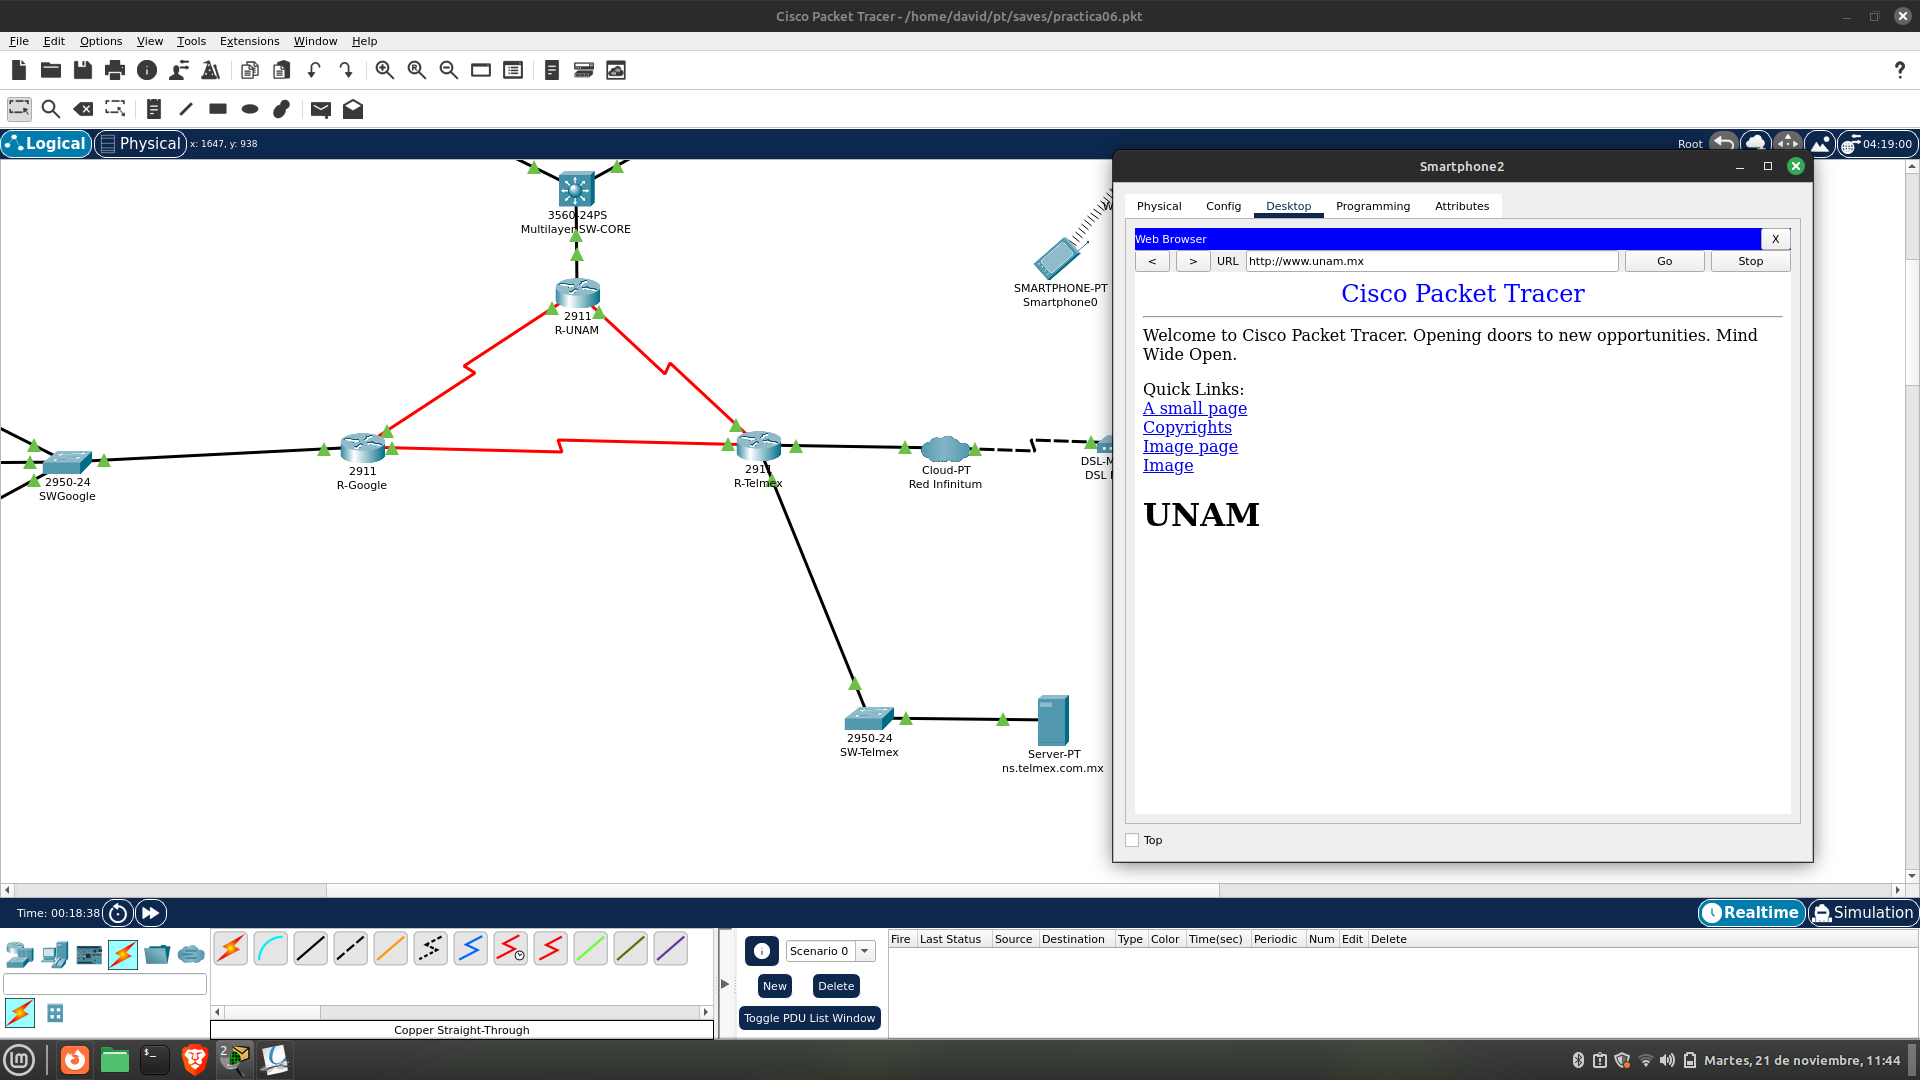
\includegraphics[width=12cm, height=8cm]{images/prueba 5 siiiiii.png} Smartphone2 a  www.unam.mx\\

\textbf{ Mostrar la memoria caché de cada servidor DNS después de haber accedido a los sitios web.}
\vspace{1em}

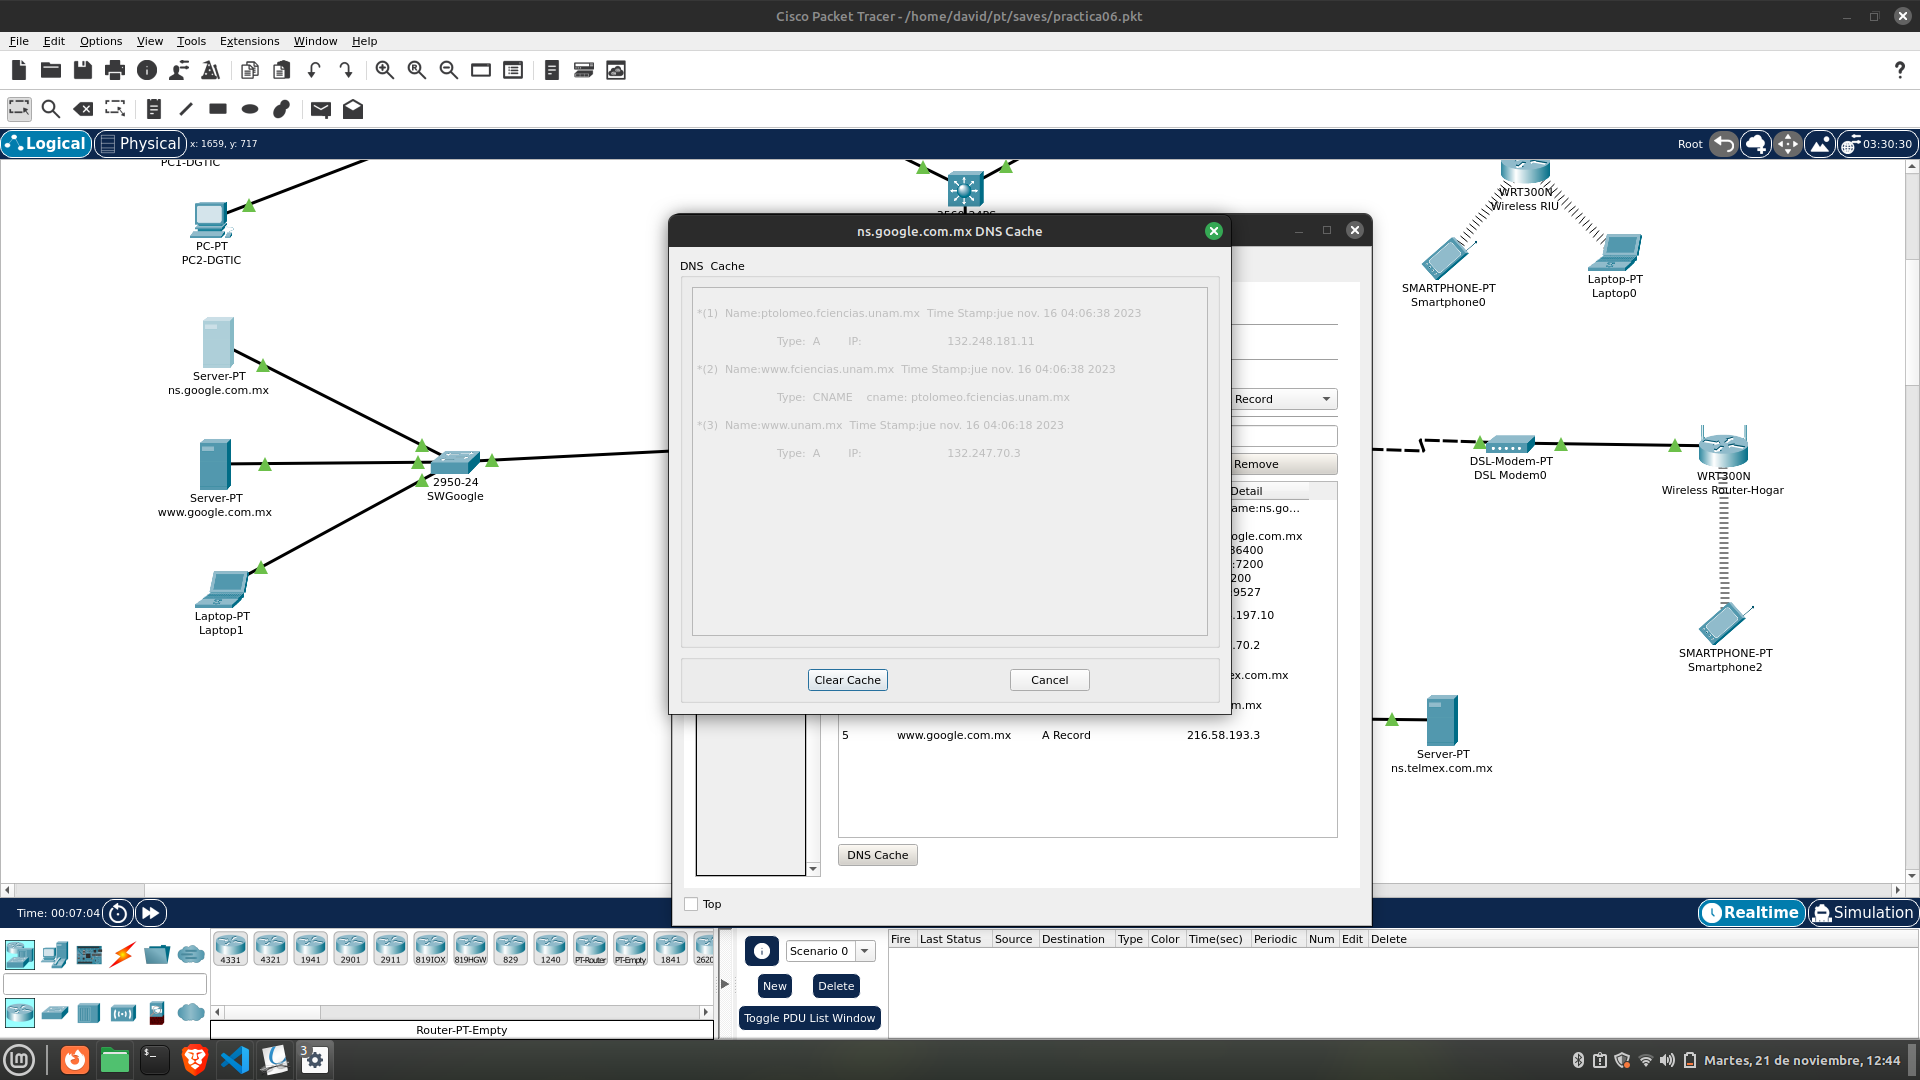
\includegraphics[width=12cm, height=8cm]{images/cache dns google.png} Memoria cache de servidor DNS de Google\\


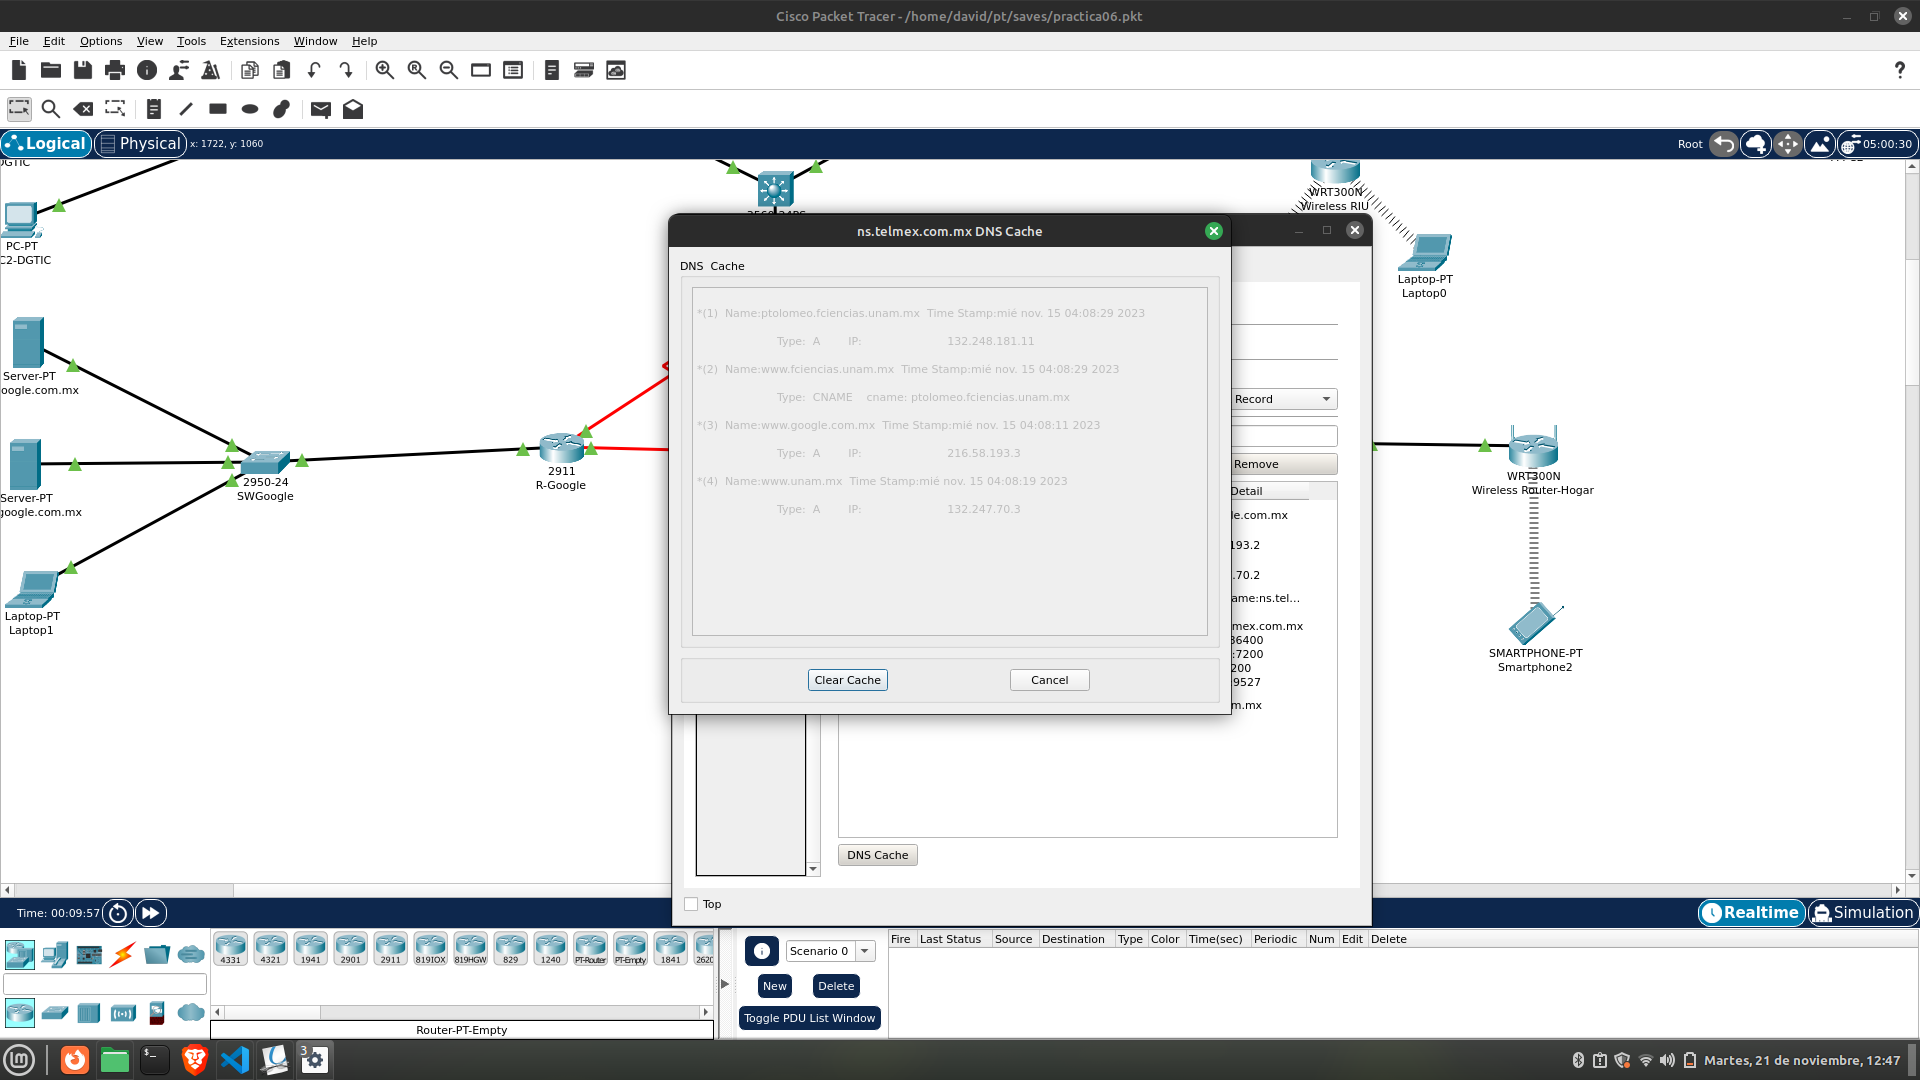
\includegraphics[width=12cm, height=8cm]{images/cache dns telmex.png} Memoria cache de servidor DNS de Telmex\\


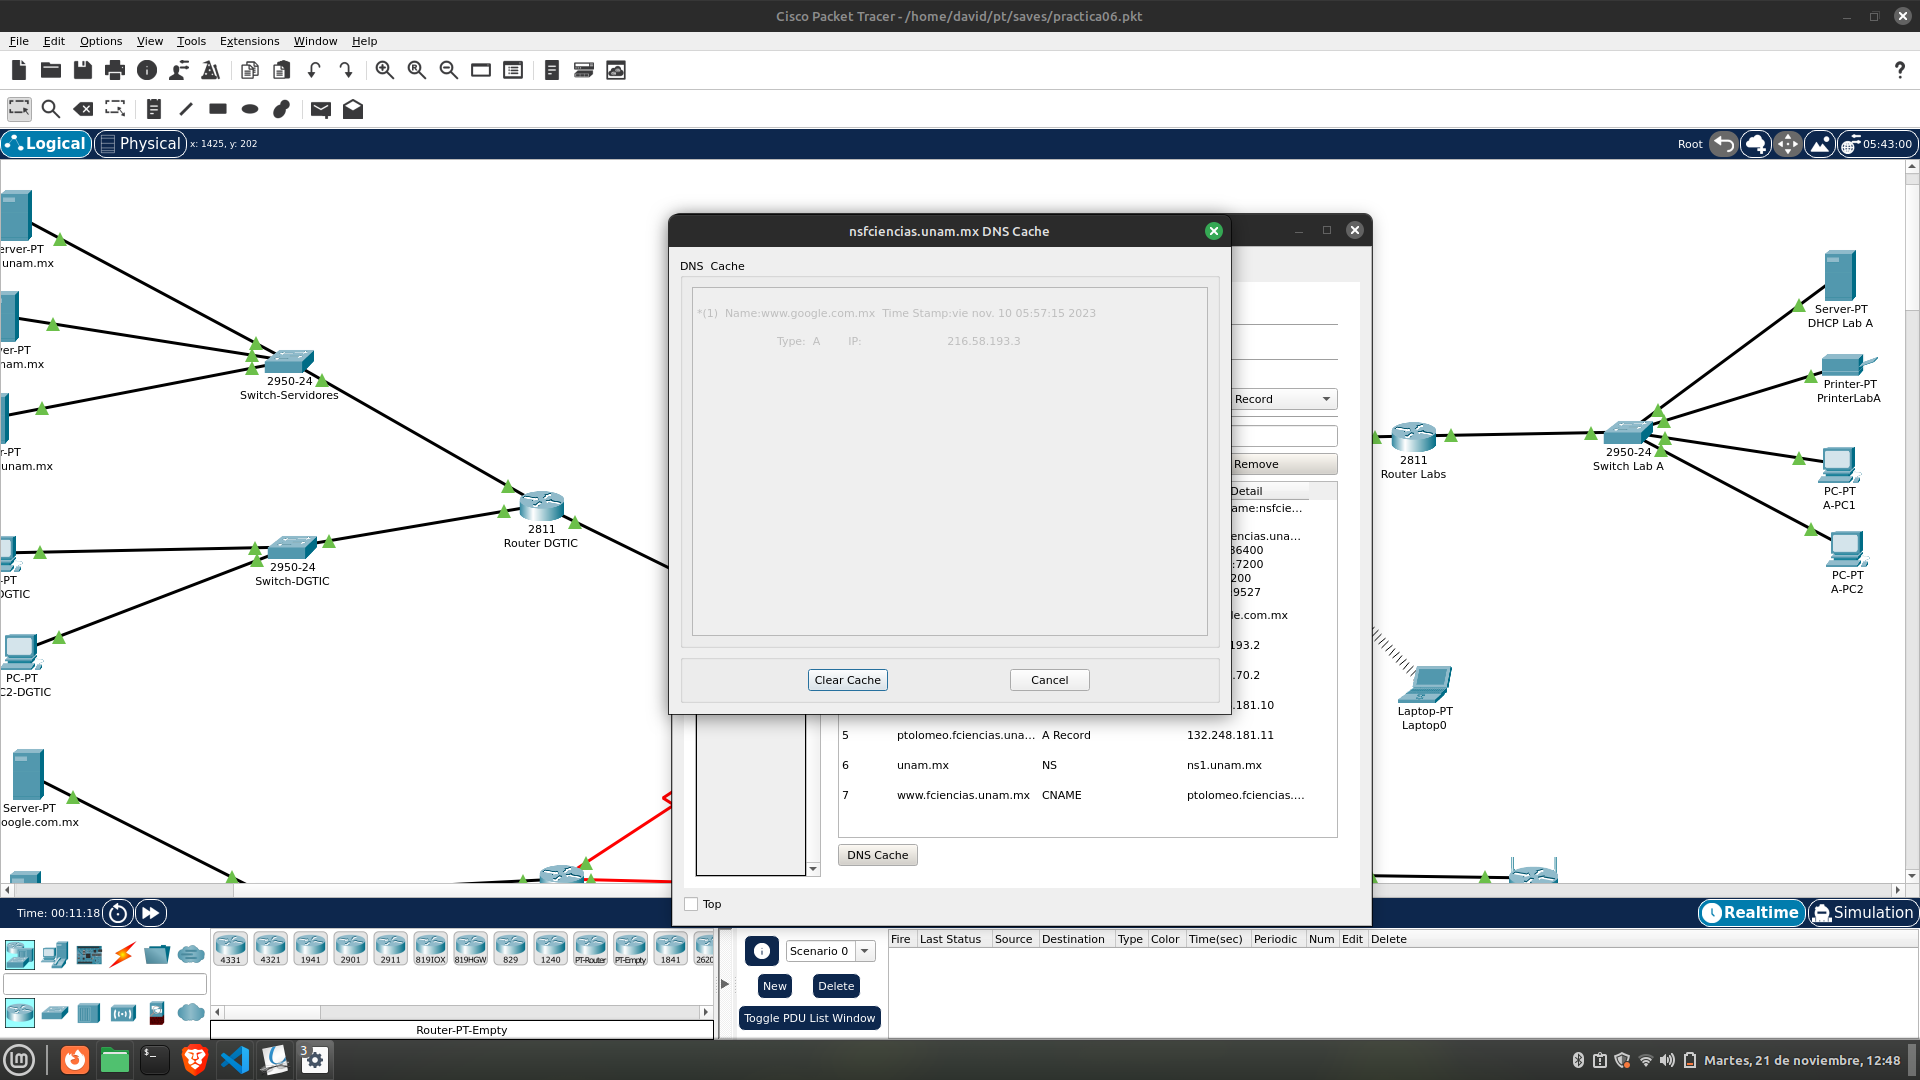
\includegraphics[width=12cm, height=8cm]{images/cache dns ciencias.png} Memoria cache de servidor DNS de fciencias\\


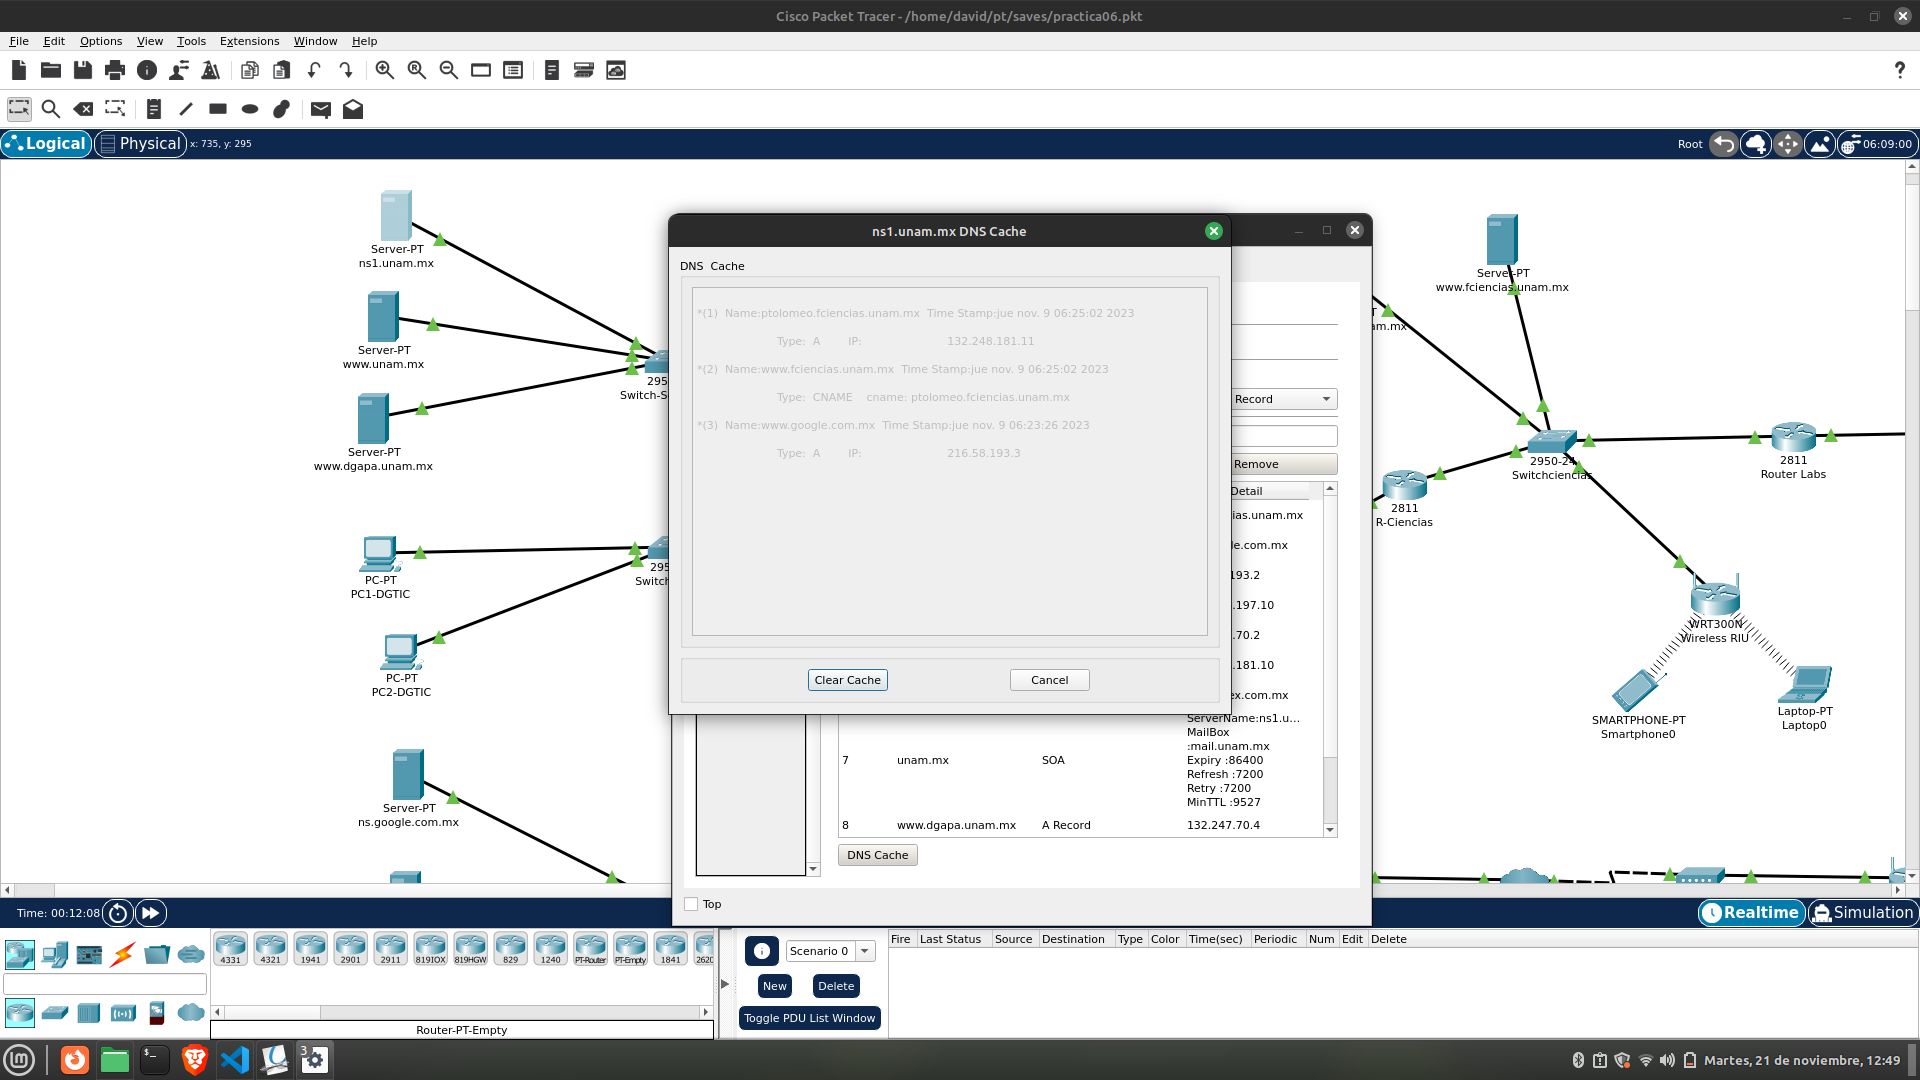
\includegraphics[width=12cm, height=8cm]{images/cache dns unam.png} Memoria cache de servidor DNS de UNAM\\


{\color{red} \subsection*{\textbf{Preguntas}}}
\vspace{1em}

\begin{enumerate}
  \item ¿Cuáles son diferencias entre las versiones 1 y 2 del protocolo RIP?\\
  \textbf{RIP v2 se diseñó para superar las limitaciones de RIP v1, proporcionando mejoras en términos de compatibilidad con IPv6, seguridad, capacidad de enrutamiento y eficiencia de transmisión de información de enrutamiento.}
  \item ¿Qué algoritmo de ruteo implementa RIP versión 2?\\
  \textbf{RIPv2 utiliza el mismo algoritmo básico que RIPv1 (distance vector routing), las mejoras y características adicionales de RIPv2, como el soporte para subredes de longitud variable (VLSM), la autenticación y el soporte para IPv6, hacen que RIPv2 sea más flexible y robusto en comparación con su predecesor.}
\end{enumerate} 

\end{document}